%!TeX root = "main.tex"

%%%%%%%%%%%%%%%%%%%%%%%%%%%%%%%%%%%%%%%%%%%%%%%%%%%%%%%%%%%%%%%
\section{Introduction}

Zero Knowledge Proofs are protocols that allow a prover to provide a proof of certain statement to a verifier revealing nothing more than the veracity of the proof itself.





%%%%%%%%%%%%%%%%%%%%%%%%%%%%%%%%%%%%%%%%%%%%%%%%%%%%%%%%%%%%%%%%%%%%%%%%%%%%%%%%
\section{Background}

%%%%%%%%%%%%%%%%%%%%%%%%%%%%%%%%%%%%%%%%%%%%%%%%%%%%%%%%%%%%%%%%%%%%%%%%%%%%%%%%
\subsection{Terminology and Conventions}

Let $n,n_1,n_2 \in \NN$ such that $n_1 < n_2$. We often denote by $[n]$ to the set $\{1,2,\dots, n\}$ and by $[n_1,n_2]$ to the set $\{n_1, n_1+1, \dots, n_2 - 1, n_2\}$.

We denote by $\FF$ to a finite field of prime order $p$ and by $\FF^*$ to its respective multiplicative group. We also write $\FF[X]$ for the ring of polynomials with coefficients over $\FF$ and write $\FF_{<d}[X]$ to denote the set of polynomials of degree lower than $d$. Given a positive integer $N$, we always assume the existence of a cyclic subgroup $G$ of $\FF^*$ and denote by $g \in \FF$ to its generator.

In PIL we treat polynomials and entire columns of execution traces indistinguishably for the following reason. Given a column $\att$ of length $N$, which can be viewed as the vector $(a_1,\dots,a_N)$ with $a_i \in \FF$ for $i \in [N]$, we define the polynomial $\att(X) \in \FF_{<N}[X]$ such that $\att(g^i) = \att_i$. Consistently, we number the rows of execution traces from $1$ to $N$. Finally, when we write constraints such as:
\[
  \att = \btt + 3,  
\]
we always refer to polynomial constraints over the corresponding group $G$, that is, the above constraint should be thought of as polynomials $\att,\btt$ satisfying $\att(g^i) = \btt(g^i) + 3$ for all $i \in [N]$. Also, unless necessary, we try to avoid the use of variables since all the polynomials that we deal with are univariate. 

% Namely, the prime\footnote{This prime is often incorrectly called a \textit{Goldilocks prime}.} $p = 2^{64} - 2^{32}+1$ is often used not only because it contains a large power of two order multiplicative subgroup, but also because the arithmetic is fast.

% Given a cyclic subgroup $S$ of $\FF^*$, we denote by $L_i \in \FF_{<|S|}[X]$ the $i$-th \textit{Lagrange polynomial} for $S$. That is, $L_i$ satisfies $L_i(g^i) = 1$ and $L_i(g^j) = 0$ for $j \neq i$, where $g$ is used here to denote the generator of $S$. Moreover, we denote by $Z_S(X) = X^{|S|} - 1 \in \FF[X]$ to the polynomial that vanishes only over $S$ and call it the \textit{vanishing polynomial} over $S$.
% It can be checked that the $i$-th Lagrange polynomial has the form:
% \[
% L_i(X) = \frac{g^i\:(X^n - 1)}{n\:(X - g^i)}.
% \]

%TODO: Just copy-paste, correct from here


%%%%%%%%%%%%%%%%%%%%%%%%%%%%%%%%%%%%%%%%%%%%%%%%%%%%%%%%%%%%%%%
\subsection{Probabilistic Proofs}

The typical scenario in VC is that the verifier, denoted $\V$, sends a program description $f$ and an input $x$ for that program to the prover, denoted $\P$. Then, $\P$ computes and returns the execution of program $f$ on input $x$, i.e., $y = f(x)$, along with a \enquote{short} proof $\pi$ that the output $y$ is correct and consistent with the description $f$ which can be efficiently verifier by $\V$. In this scenario, the computation $f$ is expressed as a set of arithmetic constraints involving $x$ and $y$. Here, arithmetic means that those constraints are equalities over a finite field $\FF$ or large prime order. Hence, $\P$ can provide proof of correctness by solving the set of constraints. As mentioned before, these constraints are equivalent to arithmetic circuits, where the gates are operations in $\FF$ and the inputs are elements from $\FF$. 

Formally, the VC proof system should satisfy the following properties:
\begin{itemize}
\item \textbf{Completeness}. If the prover $\P$ is honest so that the claim $f(x) = y$ is true, then $\P$ should be able to compute a proof that convinces the verifier $\V$ of the validity of the claim.

\item \textbf{Soundness}. A malicious prover $\P'$ should not be able to produce proof that convinces a verifier $\V$ of a statement of the form $f(x) = y'$, where $y' \neq y$. 
\end{itemize}

To also make the aforementioned short proofs privacy-preserving, $\P$ can provide his private input $w$ to the computation, known as the \textit{witness}. Thus, $f$ now is written as a function of two inputs such that $f(x,w) = y$. If at the end of the protocol, $\V$ is convinced that the statement $y = f(x,w)$ is true without learning anything about $w$, then the scheme is a ZKP. Most existing works leverage ACs where the algorithm is transformed to constraints and the proof convinces $\V$ that $\P$ knows a witness satisfying these constraints. 

More formally, a VC-proof system is said to be ZKP if the zero-knowledge property is also satisfied by the VC:
\begin{itemize}
\item \textbf{Zero-Knowledge}: After interacting with the prover $\P$ about the claim $f(x,w) = y$, $\V$ should learn nothing about the witness $w$ and still be convinced of the validity of the claim.
\end{itemize}

%%%%%%%%%%%%%%%%%%%%%%%%%%%%%%%%%%%%%%%%%%%%%%%%%%%%%%%%%%%%%%%
\subsection{Constraint System: eAIR}

In this section, we recall the constraint system eAIRs of \cite{eSTARK}. An eAIR is an extension of AIR in which not only identity constraints are available. More specifically, eAIR adds three new types of identities based on well-known arguments: permutation argument, inclusion argument and connection argument. 

\begin{table}[H]
\centering
\begin{tabular}{|c|c|c|}
\hline
\textbf{PIL Symbol} & \textbf{Type} & \textbf{Protocol} \\\hline
\tt{=} & Identity & ZeroCheck \\\hline
\tt{is} & Permutation & \cite{EPRINT:GabWilCio19} \\\hline
\tt{in} & Inclusion & Plookup \cite{EPRINT:GabWil20} \\\hline
\tt{connect} & Connnection & \cite{EPRINT:GabWilCio19} \\\hline
\end{tabular}
\caption{TBD}
\label{fig:TBDDD}
\end{table}

The eAIR constraint system aims to be as generic as possible and in particular, it captures both register machines and arithmetic circuits.

%TODO: Find a name for our model
Our hardware model will be a simple register machine with \textit{read-only} memory access. This means that the state of the machine will be represented by a fixed number of registers and the evolution of this state will be determined by a function $f$ that takes both the values stored in the registers and the data stored in the memory as inputs. However, there is one important consideration: the input to the function $f$ at the state representing the ``first'' step must coincide with the output of $f$ having as input the state representing the ``last'' step\footnote{Equivalently, $f$ establishes a relationship between each pair of consecutive states, and as a result, we must also enforce this relationship to hold between the ``last'' and the ``first'' state.}. We will explain this in more detail later on. See Figure \ref{fig:comp-model} for an image representation of this model.
\begin{figure}[H]
    \centering
    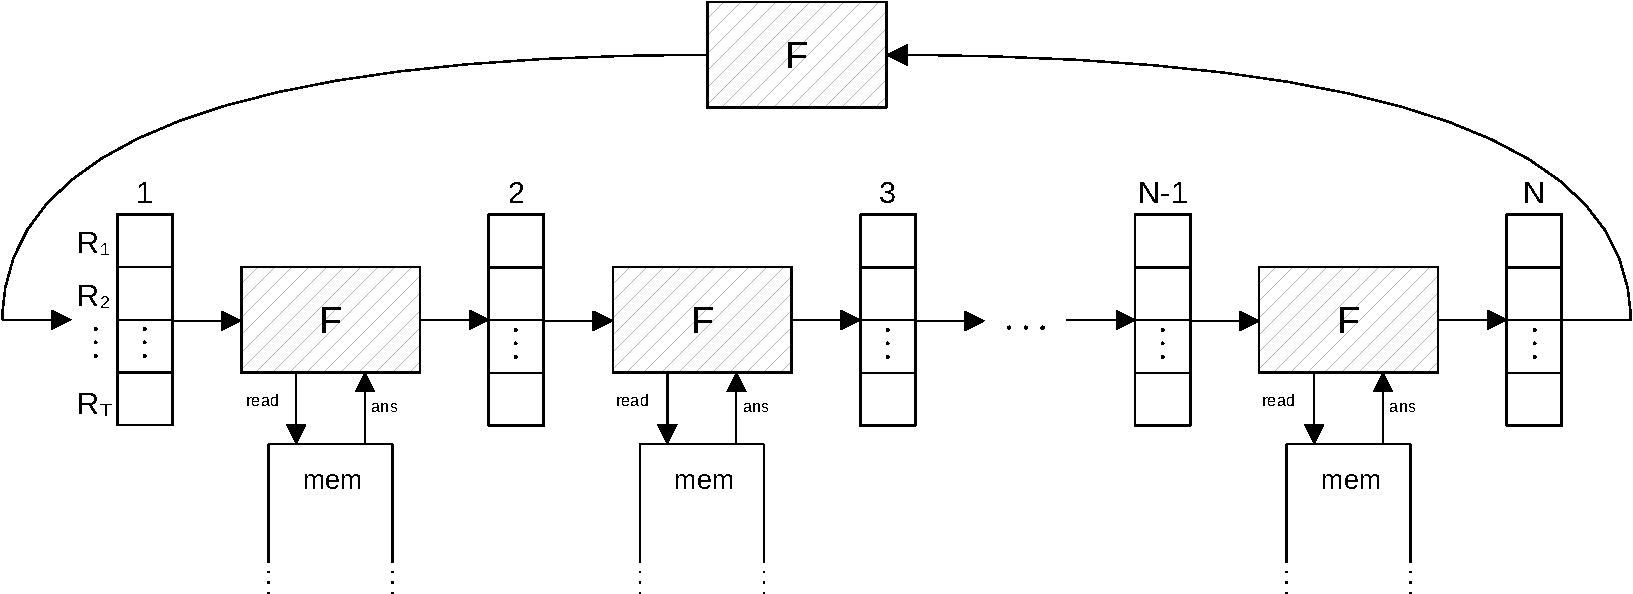
\includegraphics[width=0.8\textwidth]{../figures/computation-memory-diagram}
    \caption{Depiction of our model with $T$ registers and $N$ steps.}
    \label{fig:comp-model}
\end{figure}

Specifically, our model is parameterized by two positive integers $(T, N)$, one representing the number of registers and the other representing the number of steps, and it consists of the following components:
\begin{enumerate}
\item \textit{Registers}. A constant number $T$ of \textit{registers} $R_1,\dots,R_T$. Registers are a set of accessible cells that are available and can be manipulated by our machine in each state transition. Each of them contains data that, unless stated otherwise, is represented by an element in $\FF$. We use $r_{i,j}$ to denote the field element that, at step $i$, is contained in register $R_j$, with $i\in[N]$ and $j \in [T]$. 
    % \begin{enumerate}[a)]
    % \item \textit{Address}: A unique, distinguishable locator equivalent to a natural number.
    
    % \item \textit{Data}: Piece of information contained within a register. Unless stated otherwise, it will hold an element in $\FF$.
    % \end{enumerate}

\item \textit{Memory}. Memory is the primary location from which the information is retrieved. The main difference between the memory and the registers is that while the memory cells can only store data, the registers can be manipulated by the machine. The memory is represented by an $N \times T$ matrix $\M = \{m_{i,j}\}_{i\in[N],j\in[T]}$ of field elements. At each step, the machine reads the corresponding row of $\M$ (that is, $T$ elements) by ``popping'' it off the memory and using it to compute the next step. 
\begin{remark}
    Notice that since our machine is read-only, the elements that are read from memory are never ``pushed'' back.
\end{remark}

% \item \textit{The Program Counter}. Every register machine will contain a special register called the program counter (PC), which tells the machine what is the next instruction to execute.

\item \textit{State Transition Function}. As mentioned before, the \textit{state} of a machine at a given point $i$ consists of the set of $T$ elements from $\FF$ that its registers hold at the $i$-th step of the computation. The machine defines a state transition function $f \colon \FF^{2T} \to \FF^T$ that updates the $i$-th state to the $(i+1)$-th state having as input both the $i$-th state and the data stored in the memory. More concretely, for each step $i \in [N-1]$, the function $f$ satisfies:
\[
f(r_{i,1},\dots,r_{i,T},m_{i,1},\dots,m_{i,T}) = (r_{i+1,1},\dots,r_{i+1,T}),
\]
and for $i = N$:
\[
f(r_{N,1},\dots,r_{N,T},m_{N,1},\dots,m_{N,T}) = (r_{1,1},\dots,r_{1,T}),
\]
i.e., $f$ ensures that the state evolves correctly and that it ``cycles back'' from the last state to the first one.

\begin{remark}
    This cyclic relation avoids the need of defining the common notions of inputs and outputs in our model. Moreover, the ordering of our model's states can be shifted in any number of positions and in both directions, so that when we refer to a first or last state we assume that an ordering has been previously fixed.
\end{remark}
\end{enumerate}

% In the following we refer to the \textit{front-end} of our model as the process of converting a computer program into its equivalent description in terms of our model. More specifically, given a program

\begin{definition}[Arithmetic Circuit]
An \textit{arithmetic circuit $C$} over a field $\FF$ is a directed acyclic graph in which input and output nodes are connected with intermediate nodes through wires. The nodes are typically called \textit{gates} and are labeled by either $+$ (a \textit{sum} gate) or $\times$ (a \textit{product} gate), with two exceptions. First, every node in it with in-degree zero is called an \textit{input gate} and is labeled by either a variable $x_i$ or an element from $\FF$. Second, every node in it with outdegree zero is called an \textit{output gate} and is labeled by a polynomial with coefficients from $\FF$.

The AC processes its input, hence obtaining a polynomial, in the following way. Starting from the input gates, their path is followed and in the process, some gates compute the sum of the polynomials computed by their children, while product gates compute the product of the polynomials computed by their children. A simple example of this process is illustrated in Fig. \ref{fig:arithmeticCircuit}.
\end{definition}

\begin{figure}[H]
\centering
\begin{tikzpicture}
% vertices
\node[vertex] (1) at  (0,0) {$+$};
\node[below left=0.5cm of 1, vertex, fill=cyan!20!white] (A) {$x_1$};
\node[below right=0.5cm of 1, vertex, fill=cyan!20!white] (B) {$x_2$};
\node[vertex] (2) at  (2,0) {$\times$};
\node[right=1.4cm of 2,,yshift=15pt] (F) {Intermediate Gates};
\node[below right=0.5cm of 2, vertex, fill=cyan!20!white] (C) {$11$};
\node[right=0.5cm of C] (E) {Input Gates};
\node[vertex] (3) at  (1,1) {$+$};
\node[above=0.5cm of 3, rectangle, draw] (D) {$(x_1 + x_2) + 11 \cdot x_2$};
\node[right=1cm of D] (G) {Output Gates};
%edges
\draw[edge] (A) to node[left,xshift=2pt,yshift=4pt]{} (1);
\draw[edge] (B) to node[right,xshift=0pt,yshift=4pt]{} (1);
\draw[edge] (B) to node[left,xshift=0pt,yshift=4pt]{} (2);
\draw[edge] (C) to node[right,xshift=0pt,yshift=4pt]{} (2);
\draw[edge] (1) to node[right,xshift=0pt,yshift=4pt]{} (3);
\draw[edge] (2) to node[right,xshift=0pt,yshift=4pt]{} (3);
\draw[edge] (3) to node[left,xshift=0pt,yshift=4pt]{} (D);
\end{tikzpicture}
\caption{Arithmetic circuit that performs two additions and one multiplication.}
\label{fig:arithmeticCircuit}
\end{figure}


%%%%%%%%%%%%%%%%%%%%%%%%%%%%%%%%%%%%%%%%%%%%%%%%%%%%%%%%%%%%%%%%%%%%%%%%%%%%%%%%
\subsection{Arithmetization: The Bridge Between PIL and our Model}

\begin{table}[H]
\centering
\begin{tabular}{|c|l|}
\hline
\textbf{PIL Keyword} & \textbf{Register Machine Equivalent} \\\hline
\tt{namespace} & Defines a new machine. \\\hline
\tt{pol commit} & Creates a new register. \\\hline
\tt{pol const} &  \\\hline
\tt{=} & Defines (a part of) the state transition function. \\\hline
\tt{pol} &  \\\hline
\tt{public} &  \\\hline
\end{tabular}
\caption{TBD}
\label{fig:TBD}
\end{table}

In this section, we introduce the basic keywords used in PIL and how they relate to our model. The starting point is the process of \textit{arithmetization} of our model. This means that to arithmetize our model, we must specify the transition function $f$ as a set of polynomial constraints over variables representing the \enquote{current} and the \enquote{next} step of the state.

\begin{definition}[Arithmetization]
    Let $\bar{X}$ be a shorthand for the sequence of formal variables $X_1,\dots, X_T$, $\bar{M}$ a shorthand for the sequence of formal variables $M_1,\dots, M_T$ and $\bar{Y}$ a shorthand for the sequence of formal variables $Y_1\dots, Y_T$. Given a state transition function $f \colon \FF^{2T} \to \FF^T$, the \textit{arithmetization of $f$} consists on computing polynomials $p_1,\dots,p_T \in \FF[\bar{X},\bar{M},\bar{Y}]$ such that for each input state $x \in \FF^{T}$, memory row $m \in \FF^T$ and next state $y \in \FF^T$, we have that:
    \[
        f(x,m) = y \quad \text{ if and only if } \quad p_i(x,m,y) = 0 \text{ for all } i \in [T].	
    \]
    % The aritmetization will be considered to be correct if, given a pair of input $x\in \FF^{2T}$ and output $y \in \FF^T$, we have that $f(x)=y$ if and only if the polynomial constraints get satisfied on this pair.
\end{definition}


% \begin{definition}[execution trace]
%     The \textit{execution trace} of our model is the matrix of $N \times T$ field elements where:
%     \begin{enumerate}
%     \item Each row $i \in [N]$ corresponds with the state of the machine at the $i$-th step.
    
%     \item Each column $j \in [T]$ corresponds with the content of the $j$-th register over every step.
%     \end{enumerate}
% \end{definition}




%%%%%%%%%%%%%%%%%%%%%%%%%%%%%%%%%%%%%%%%%%%%%%%%%%%%%%%%%%%%%%%%%%%%%%%%%%%%%%%%
\subsection{Register Machine Relation}



%%%%%%%%%%%%%%%%%%%%%%%%%%%%%%%%%%%%%%%%%%%%%%%%%%%%%%%%%%%%%%%
\subsection{Related Work}

The main objective of STARK-based languages is translating a computation described as a computer program to a computation described as an AIR. The distinct ways this process can be achieved can be divided into two:
\begin{enumerate}
    \item \textbf{ASIC-like}: This approach is based on writing a computer program in some domain-specific language (DSL) that compiles to an equivalent AIR representing the satisfiability of the computer program. Examples of such are PIL itself and AirScript \cite{AirScript}.
    \item \textbf{CPU-like}: This approach attempts to design an AIR that behaves like a CPU that can handle any computation passed to it. This means that a program is no longer directly compiled into AIR. Instead, the program is compiled to a reduced set of assembly instructions that are understood by the CPU and then the assembly program is transformed to the single AIR representing the correct execution of the CPU. Examples of such are Zilch \cite{EPRINT:MouTso20} and Cairo \cite{EPRINT:GolPapRia21}.
\end{enumerate}

None of the previous variants is the best for every computer program we can think of, as they present several advantages and disadvantages depending on the particular program they are dealing with. Even if more involved, we preferred the ASIC-like approach for PIL for the following reasons:
\begin{enumerate}[a)]
    \item Efficiency: Since the AIR is dependent on the specific computer program, one can design an AIR tailored to that program. In particular, one can decide whether his design is based on a ``wider'' and ``shorter'' or on a ``thinner'' and ``higher'' execution trace.
    \item Modularity: One can divide a program into multiple small pieces (relating these pieces appropriately) and produce an AIR for each piece separately that will ultimately produce an AIR for the entire program. This allows the user to build a vast program through handle (small) logic. 
\end{enumerate}

Similar to PIL, AirScript is a DSL to produce AIR constraints in an ASIC-like fashion. The main problem of AirScript is that it has very little abstraction for describing non-identity constraints. While PIL has built-in keywords for such constraints (that could be augmented in the future), an AirScript user needs to deal with them explicitly: for any argument that is based on random field elements supplied by the verifier during the protocol, a user must define identity constraints attesting the argument's validity by accessing the verifier's randomness. For example, if one wants to produce a program checking that a column is a value in the range $[0,2^4-1]$ by using the Plookup \cite{EPRINT:GabWil20} inclusion argument (in the style described in \cite{EPRINT:PFMBM22}):
\begin{pil}
namespace Example();
    pol commit a;
    pol constant BITS4;

    a in BITS4;
\end{pil}
\begin{pil}
def Example
    trace_columns:
        main: [a,BITS4,h1,h2]
        aux: [Z]

    boundary_constraints:
        enf Z.first = 1

    integrity_constraints:
        enf Z'*($rand[0]*(1+$rand[1])+h1+$rand[1]*h2)*($rand[0]*(1+$rand[1])+h2+$rand[1]*h1') = Z*(1+$rand[0])*($rand[1]+a)*($rand[0]*(1+$rand[1])+BITS4+$rand[1]*BITS4')
\end{pil}
Even tho more generic, an AirScript user must choose and understand the argument he wants to deal with, making it less attractive than PIL to the public. 

Regarding CPU-like approaches like Zilch and Cairo, they are both based on a similar workflow: (1) write a program for the computation (either using an assembly-like language directly or using any other language that can be compiled to the CPU bytecode); (2) compile the program to the CPU bytecode; and (3) use a STARK prover for the single AIR to generate a proof. This two-step paradigm suffers from efficiency, as the set of assembly instructions is unlikely to be optimal for every single program. Therefore, while step (3) is independent of the specific program that the user deals with (something that appears to be very handy in proof systems), this does not justify the overhead generated in step (2) as vast programs might have an untractable bytecode whose proof might take too long to compute for practical deployment.


%%%%%%%%%%%%%%%%%%%%%%%%%%%%%%%%%%%%%%%%%%%%%%%%%%%%%%%%%%%%%%%%
\subsection{Arguments}\label{sec:preliminaries:arguments}

In this section, we introduce the ``arguments'' that have their keyword in PIL. Here, by argument, we mean a relation between polynomials that cannot be directly expressed through an identity. We often refer to them more naturally as \textit{non-identity constraint}. The three arguments we will introduce are \textit{permutation}, \textit{connection} and \textit{inclusion}.

The protocols that instantiate these arguments are all based on the same idea of the computation of a grand-product polynomial over the two (or more) vectors involved in the argument. Specifically, a polynomial is cumulatively computed as the quotient of a function of the first vector and a function of the second vector. Then, a set of identities is proposed as insurance for a verifier of the protocol that not only the grand product was correctly computed by a prover, but also that the specific intention of the protocol is satisfied. To ensure the soundness of the protocols, random values uniformly sampled by the verifier are used in such computation.

An alternative to the previous idea is based on the addition of logarithmic derivatives (see e.g. \cite{EPRINT:Habock22M}) instead, but they come with tradeoffs that make them unwanted for the STARK context. 

Recall that $G = \langle g \rangle$ is a cyclic subgroup of $\FF^*$ of order $n$.

%TODO: Should we call it vector equality argument?
%%%%%%%%%%%%%%%%%%%%%%%%%%%%%%%%%%%%%%%%%%%%%%%%%%%%%%%%%%%%%%%%
\subsubsection*{Permutation}

Given two vectors $f = (f_1, \dots, f_n)$ and $t = (t_1, \dots, t_n)$ in $\FF^n$, a permutation argument, denoted $f \doteq t$, is used for checking that $f$ and $t$ are a permutation of each other. The protocol that instantiates the permutation arguments works by computing the following grand-product polynomial $Z \in \FF_{<n}[X]$:
\[
  Z(g^i) = 
  \begin{cases} 
  1, & \text{if }~ i=1 \\ 
  \displaystyle\prod_{j=1}^{i-1} \frac{(f_j + \gamma)}{(t_j + \gamma)}, & \text{if }~ i = 2, \dots, n
  \end{cases} 
\]
where $\gamma \in \FF$ is the value sent from the verifier. 

The definition of the previous polynomial is based on the following lemma.
\begin{lemma}[Soundness of Permutation]\label{lemma:muleq-soundness}
  Fix two vectors $f = (f_1, \dots, f_n)$ and $t = (t_1, \dots, t_n)$ in $\FF^n$. If the following holds with probability larger than $n/|\FF|$ over a random $\gamma \in \FF$:
  \begin{equation*}
  \prod_{i=1}^n (f_i + \gamma) = \prod_{i=1}^n (t_i + \gamma),
  \end{equation*}
  then $f \doteq t$. 
\end{lemma}

As a consequence of Lemma \ref{lemma:muleq-soundness}, the identities that must be checked by the verifier for $x \in G$ are the following: 
\begin{align*}
&L_1(x) \cdot (Z(x) - 1) = 0, \\
&Z(x \cdot g) \cdot (t(x) + \gamma) = Z(x) \cdot (f(x) + \gamma),
\end{align*}
where $f,t \in \FF_{<n}[X]$ are the polynomials resulting from the interpolation of $\{f_i\}_{i\in[n]}$ and $\{t_i\}_{i\in[n]}$ over $G$,respectively.




%%%%%%%%%%%%%%%%%%%%%%%%%%%%%%%%%%%%%%%%%%%%%%%%%%%%%%%%%%%%%%%%
\subsubsection*{Connection}

The protocol for a connection argument and the definitions and results we provide next are adapted from \cite{EPRINT:GabWilCio19}.

Given some vectors $f_1,\dots,f_k \in \FF^n$ and a partition $\T = \{T_1,\dots,T_k\}$ of the set $[k] \times [n]$, a connection argument, denoted $(f_1,\dots,f_k) \propto \{T_1,\dots,T_k\}$, is used to check that the partition $\T$ divides the field elements $\{f_{i,j}\}_{i\in[k],j\in[n]}$ into sets with the same value. More specifically, we have $f_{i_1,j_1} = f_{i_2,j_2}$ if and only if $(i_1,j_1),(i_2,j_2)$ belong to the same block of $\T$. 

To express the partition $\T$ within a grand-product polynomial, we define a permutation $\sigma\colon [kn] \to [kn]$ as follows: $\sigma$ is such that for each block $T_i$ of $\T$, $\sigma(\T)$ contains a cycle going over all elements of $T_i$. Then, the protocol that instantiates the connection arguments works by computing the following grand-product polynomial $Z \in \FF_{<n}[X]$:
\[
  Z(g^i) = 
  \begin{cases} 
  1, & \text{if }~ i=1 \\ 
  \displaystyle\prod_{\ell=1}^{k}\prod_{j=1}^{i-1} \frac{(f_{\ell,j} + \gamma \cdot (\ell-1)\cdot n +j) + \delta)}{(f_{\ell,j} + \gamma \cdot \sigma((\ell-1)\cdot n +j) + \delta)}, & \text{if }~ i = 2, \dots, n
  \end{cases} 
\]
where $\gamma,\delta \in \FF$ are the values sent from the verifier. 


The definition of the previous polynomial is based on the following lemma, a proof of which can be found\footnote{The claim in \cite{EPRINT:GabWilCio19} is for a slightly more general protocol.} in Claim A.1. of \cite{EPRINT:GabWilCio19} and is similar to the one of Lemma \ref{lemma:muleq-soundness}.
\begin{lemma}[Soundness of Connection]\label{lemma:connection-soundness}
Fix $f_1,\dots,f_k \in \FF^n$ and a partition $\T = \{T_1,\dots,T_k\}$ of $[k] \times [n]$. If the following holds with probability larger than $kn/|\FF|$ over randoms $\gamma, \delta \in \FF$:
\[
\prod_{\ell=1}^k \prod_{j=1}^n (f_{\ell,j} + \gamma \cdot ((\ell-1)\cdot n + j) + \delta) = \prod_{\ell=1}^k \prod_{j=1}^n (f_{\ell,j} + \gamma \cdot \sigma((\ell-1)\cdot n + j) + \delta),
\]
then, $(f_1,\dots,f_k) \propto \{T_1,\dots,T_k\}$.
\end{lemma}

As a consequence of Lemma \ref{lemma:connection-soundness}, the identities that must be checked by the verifier for $x \in G$ are the following: 
\begin{align*}
\begin{array}{c}
  L_1(x) \cdot (Z(x) - 1) = 0, \\[0.2cm]
  \displaystyle Z(x \cdot g)  = Z(x) \cdot \frac{(f_{1}(x) + \gamma \cdot S_{\ID_1}(x) + \delta)}{(f_{1}(x) + \gamma \cdot S_{\sigma_1}(x) + \delta)} \cdot \cdots \cdot \frac{(f_{k}(x) + \gamma \cdot S_{\ID_k}(x) + \delta)}{(f_{k}(x) + \gamma \cdot S_{\sigma_k}(x) + \delta)},
\end{array}
\end{align*}
where $S_{\ID_{\ell}}(g^j) = (\ell-1)\cdot n +j$ is the polynomial mapping $G$-elements to indexes in $[kn]$ and $S_{\sigma_{\ell}}(g^j) = \sigma((\ell-1)\cdot n +j)$ is the polynomial defined by $\sigma$. Since the permutation $\sigma$ perfectly relates with the partition $\T$ it refers to, from now on we denote a connection argument between polynomials $f_1,\dots,f_k \in \FF[X]$ and a partition $\T$ as $(f_1,\dots,f_k) \propto (S_{\sigma_1},\dots, S_{\sigma_k})$. As we will see in later sections, this overloading notation will become very natural.

For more details see \cite{EPRINT:GabWilCio19}.

%Permutations
In this section, a new kind of constraint that can be used in PIL will be introduced: \textbf{permutation arguments}. Previously inclusion checks have been described. However, permutation arguments are much stronger arguments. 

\begin{definition}
Given two vectors $a = (a_1, \dots, a_n)$ and $b = (b_1, \dots, b_n)$, we say that $a$ is a permutation of $b$ (or conversely) if there exists a permutation (that is, a bijective map $\sigma: \{1, \dots, n\} \to \{1, \dots, n\})$ such that $a = \sigma(b)$ where $\sigma(b)$ is defined as
\[
\sigma(b) := (b_{\sigma(1)}, \dots, b_{\sigma(n)}).
\]
\end{definition}

Observe that unlike inclusion arguments both vectors must have the same length: 

To see some specific examples, observe that
\begin{align*}
&(3, 2) \subset (1, 2, 3, 4) \\
&(1, 5, 5, 5, 8, 1, 1, 2) \subset (1, 2, 4, 5, 8) \\
&(3, 2, 3, 1) \text{ is a permutation of } (1, 2, 3, 3) \\
&(5, 5, 6, 9, 0) \text{ is a permutation of } (6, 5, 9, 0, 5)
\end{align*}

As a final and important remark, the \SEL column should be turned on the same amount of times in both programs. Otherwise, a permutation can not exist between any of the columns. This allows us to use this kind of argument even if both tables do not have the same amount of rows. Another way of saying it, is permutation arguments check bijective maps from rows to rows, which also prohibits many-to-one or one-to-many assignments which can be treated with inclusion arguments. On the other hand, if in the design of the connection between both programs, we expect one-to-one correspondence among them, we can simply drop both \SEL columns, similar to what we have done previously with the inclusion arguments. To sum up, with an explicit example, observe that the following two execution traces can not be related with a permutation argument but a inclusion one:

\vspace{.5cm}
\begin{tabular}{ c c c }
    
\begin{tabular}{|c|c|c|c|c|c|c|}
\hline
\multicolumn{7}{|c|}{\textbf{Program A}} \\
\hline
\textbf{\dots} &$\sel$	&$\att$	&$\btt$	&\textbf{\dots}	&$\ctt$	&\textbf{\dots}	\\ \hline
\dots	&1	&1	&2	&\dots	&7	&\dots \\
\dots	&1	&3	&5	&\dots	&2	&\dots \\
\hline
\end{tabular}

\quad 

\begin{tabular}{|c|c|c|c|c|c|c|}
\hline
\multicolumn{7}{|c|}{\textbf{Program B}} \\
\hline
\textbf{\dots} &$\sel$	&$\mathtt{d}$	&$\mathtt{e}$	&\textbf{\dots}	&$\mathtt{f}$	&\textbf{\dots}	\\ \hline
\dots	&0	&9	&6	&\dots	&6	&\dots \\
\dots	&1	&2	&1	&\dots	&7	&\dots \\
\dots	&1	&5	&3	&\dots	&2	&\dots \\
\dots	&0	&3	&3	&\dots	&3	&\dots \\
\dots	&1	&2	&1	&\dots	&7	&\dots \\
\hline
\end{tabular}
\end{tabular}
\vspace{.5cm}

Let us exemplify how to use a permutation argument using the example started in section \ref{sec:connecting-sm}. 


%Connections
In this section, a new kind of constraint that can be used in PIL will be introduced: \textbf{connection arguments}. Suppose that we are given a vector $a = (a_1, \dots, a_n)$ and a partition $S$ of $\{1, \dots, n\}$. Recall that a partition $S$ of a set $X$ is a set of non-empty subsets of $X$ such that every element $x$ in $X$ is in exactly one of these subsets. We want to check that, for each $s \in S$ we have that $a_i = a_j$ whenever $i, j \in s$. This check is reminiscent of the copy constraints appearing in \plonk and, because of this, it is called connection check. Let us show a specific example. Let $S = \{ \{2\}, \{1, 3, 5\}, \{4, 6\}\}$ be the specified partition of $\{1, 2, 3, 4, 5, 6\}$. Observe the two vectors depicted below:

\begin{figure}[H]
\centering
\begin{tabular}{|c|}
\hline
\att \\ \hline
\cellcolor{cyan} 3 \\
9 \\
\cellcolor{cyan} 3 \\
1 \\
\cellcolor{cyan} 3 \\
1 \\
\hline
\end{tabular}
\begin{tabular}{|c|}
\hline
\btt \\ \hline
\cellcolor{cyan} 3 \\
9 \\
\cellcolor{red} 7 \\
1 \\
\cellcolor{cyan} 3 \\
1 \\
\hline
\end{tabular}
\caption{Example of non-satisfied connection argument. }
\label{table:connection-arg-example}
\end{figure}

The vector \att fulfills the statement defined before because $a_1 = a_3 = a_5 = 3$ and $a_4 = a_6 = 1$. Observe that, since $\{2\}$ is a singleton in $S$, $a_2$ is unconstrained and hence, can take any value. This is a general fact, if we want not to restrict the value of the position $i$ of a vector, we should include $\{i\}$ as a singleton in the partition $S$. However, in the vector \btt the connection check is not satisfied because $a_1 = a_5 = 3 \neq 7 = a_3$.

In the programs' context, connection arguments can be easily implemented in PIL by introducing a constant column associated with the chosen partition. Recall that column values are, in fact, evaluations of a polynomial at $G = \Angle{g}$, where $N$ is the length of the execution trace. Suppose we are given a polynomial $a$ and partition $S$ and we want to invoke its corresponding connection check. We will construct, for each $s = \{s_1, s_2, \dots, s_k \} \in S$, the permutation $\sigma_s = (s_k, s_1, s_2, \dots, s_{k-1})$ which is simply a 1 position rotation. That is, $\sigma_s(s_i) = s_{i+1}$. Posteriorly, we construct a polynomial $S(a)$ defined as follows:

\[
S(a)(g^i) = g^{\sigma_s(i) - 1}
\]

where $s$ is the set of the partition $S$ where $i$ belongs. Observe that we are subtracting $1$ in order to shift the set $\{1, \dots, N\}$ to $\{0, \dots, N-1\}$ which is where powers of the root of unity $g$ are well-corresponded. 


%%%%%%%%%%%%%%%%%%%%%%%%%%%%%%%%%%%%%%%%%%%%%%%%%%%%%%%%%%%%%%%%
\subsubsection*{Inclusion}

The protocol for an inclusion argument and the definitions and results we provide next are adapted from \cite{EPRINT:GabWil20}, with the ``alternating method''  provided in \cite{EPRINT:PFMBM22}.

Given two vectors $f = (f_1, \dots, f_n)$ and $t = (t_1, \dots, t_n)$ in $\FF^n$, a inclusion argument, denoted $f \in t$, is used for checking that the set $A$ formed with the values $\{f_i\}_{i\in[n]}$ is contained in the set $B$ formed with the values $\{t\}_{i\in[n]}$. Notice that $|A|,|B|\leq n$.

In the protocol, the prover has to construct an auxiliary vector $s = (s_1, \dots, s_{2n})$ containing every element of $f$ and $t$ where the order of appearance is the same as in $t$.
The main idea behind the protocol is that if $f \in t$, then $f$ contributes to $s$ with repeated elements.
To check this fact, a vector $\Delta{s}$ is defined as follows:
\[
\Delta{s} = (s_1+\gamma\,s_2, s_2+\gamma\,s_3, \cdots, s_{2n}+\gamma\,s_1).
\]

Then, the protocol essentially checks that $\Delta{s}$ is consistent with the elements of $f$, $t$ and $s$.
To do so, the vector $s$ is split into two vectors $h_1,h_2 \in \FF^n$.
In the protocol described in \cite{EPRINT:GabWil20},
$h_1$ and $h_2$ contain the lower and upper halves of $s$, while in our protocol in \cite{EPRINT:PFMBM22}, we use $h_1$ to store elements with odd indexes and $h_2$ for even indexes, that is:
\begin{equation}\label{eq:alternating-method}
h_1 = (s_1, s_3, s_5, ..., s_{2n-1}) \quad\text{ and }\quad
h_2 = (s_2, s_4, s_6, ..., s_{2n}).
\end{equation}

With this setting in mind, the grand-product polynomial is defined as:
\[
  Z(g^i) = 
  \begin{cases} 
  1, & \text{if }~ i=1 \\ 
  \displaystyle (1+\gamma)^{i-1}\prod_{j=1}^{i-1}\frac{{(\delta + f_j)}   (\delta(1+\gamma) + t_j + \gamma t_{j+1})}{ (\delta(1+\gamma) + s_{2j-1} + \gamma s_{2j})(\delta(1+\gamma) + s_{2j} + \gamma s_{2j+1})}, & \text{if }~ i = 2, \dots, n
  \end{cases} 
\]
where $\gamma,\delta \in \FF$ are the values sent from the verifier.

The definition of the previous polynomial is based on the following lemma, which is a slight modification of Claim 3.1. of \cite{EPRINT:GabWil20}.
\begin{lemma}[Soundness of Inclusion]\label{lemma:inclusion-soundness}
  Fix three vectors $f = (f_1, \dots, f_n),t = (t_1, \dots, t_n)$ and $s = (s_1,\dots,s_{2n})$ with elements in $\FF$. If the following holds with probability larger than $(4n-2)/|\FF|$ over randoms $\gamma, \delta \in \FF$:
  \begin{equation*}
    (1+\gamma)^n\prod_{i=1}^n (\delta + f_i)\prod_{i=1}^{n-1} (\delta(1+\gamma) + t_i + \gamma t_{i+1}) = \prod_{i=1}^{2n-1} (\delta(1+\gamma) + s_i + \gamma s_{i+1}),
  \end{equation*}
  then $f \in t$ and $s$ is the sorted by $t$ concatenation of $f$ and $t$. 
\end{lemma}

As a consequence of Lemma \ref{lemma:inclusion-soundness}, the identities that must be checked by the verifier for $x \in G$ are the following: 
\begin{align*}
\begin{array}{c}
  L_1(x) \left( Z(x) - 1\right) = 0, \\[0.2cm]
  Z(x\cdot g) = \displaystyle Z(x)\frac{(1+\gamma)(\delta + f(x))(\delta(1+\gamma) + t(x) + \gamma t(gx))}{(\delta(1+\gamma) + {h_1}(x) + \gamma {h_2}(x))(\delta(1+\gamma) + {h_2}(x) + \gamma {h_1}(x\cdot g))}.
\end{array}
\end{align*}
where $f,t \in \FF_{<n}[X]$ are the polynomials resulting from the interpolation of $\{f_i\}_{i\in[n]}$ and $\{t_i\}_{i\in[n]}$ over $G$, respectively; and $h_1,h_2 \in \FF_{<n}[X]$ are the polynomials resulting from the interpolation of the values defined in Eq. \eqref{eq:alternating-method} over $G$.

For more details see \cite{EPRINT:GabWil20} and \cite{EPRINT:PFMBM22}.

%inclusions
\begin{definition}
Let $a = (a_1, \dots, a_n) \in \FF_p^n$ and $b = (b_1, \dots, b_m) \in \FF_p^m$ (with no explicit relationship between $n$ and $m$) be two vectors. We say that $a \subset b$ if $a_i \in b$ for all $i \in \{1, \dots, n\}$. That is, there exists a $j \in \{1, \dots, n\}$ such that $a_i = b_j$. 
\end{definition}

An inclusion argument is a constraint defined in PIL that is used to check whether $\att \subset \btt$ where \att and \btt are two columns. Since polynomials can be described as vectors via the usual Fourier transform procedure, the following definition can be naturally extended to columns. It is important to observe that $n$ can be less, equal or bigger than $m$ and the former definition still makes sense. Later on, a more restrictive constraint will be introduced.


%%%%%%%%%%%%%%%%%%%%%%%%%%%%%%%%%%%%%%%%%%%%%%%%%%%%%%%%%%%%%%%
\section{The Language}


%%%%%%%%%%%%%%%%%%%%%%%%%%%%%%%%%%%%%%%%%%%%%%%%%%%%%%%%%%%%%%%
\subsection{Introduction}

Polynomial Identity Language (PIL) is a novel domain-specific language useful for defining eAIR constraints. The aim of creating PIL is to provide developers with a holistic framework for both constructing programs through an easy-to-use interface and abstracting the complexity of the proving mechanisms.

One of the main peculiarities of PIL is its modularity, which allows programmers to define parametrizable programs, called \texttt{namespaces}, which can be instantiated from larger programs. Building programs in a modular manner makes it easier to test, review, audit and formally verify even large and complex programs. In this regard, by using PIL, developers can create their own custom namespaces or instantiate namespaces from some public library.

Many other domain-specific languages (DSL) or tool stacks, such as Circom or Halo2, focus on the abstraction of a particular computational model, such as an arithmetic circuit. However, recent proof systems such as STARKs have shown that arithmetic circuits might not be the best computational models in all use cases. Given a complete programming language, computing a valid proof for a circuit satisfiability problem, may result in long proving times due to the overhead of re-used logic. Opting for the deployment of programs, with their low-level programming, shorter proving times are attainable, especially with the advent of proof/verification-aiding languages such as PIL.









%%%%%%%%%%%%%%%%%%%%%%%%%%%%%%%%%%%%%%%%%%%%%%%%%%%%%%%%%%%%%%%
\subsection{Creating a Simple Program}\label{sec:simple-program}

To describe the fundamentals of the language itself, let us create a simple PIL program that models the computation of the product of two integers. Consider a program that, at each step, takes two input numbers and multiplies them. Naturally, this program will be referred to as the \Multiplier program. 
% It is important to recall that multiplication is defined over some (large) finite field. 
This program can be modeled using $3$ polynomials: $2$ referring to the inputs that are going to be multiplied $\freeIn_1, \freeIn_2$, and $1$ referring to the output of the computation itself $\out$. As it can be observed, the output column will exhibit a correct behavior if and only if the following identity is satisfied:
\[
\out = \freeIn_1 \cdot \freeIn_2.
\] 

A concrete example of a correct execution trace of the \Multiplier program can be seen in Figure \ref{table:multiplier-ex}. The relation above is satisfied in each of the rows of the execution trace, which means that the output column is filled with correct values. 
\begin{figure}[H]
\centering
\begin{tabular}{|c|}
\hline
\row\\ \hline
1			\\
2			\\
3			\\
4			\\
5			\\
6			\\
\vdots			\\
\hline
\end{tabular}
\begin{tabular}{|c|c|c|}
\hline
$\freeIn_1$	& $\freeIn_2$		& \out 	\\
\hline
4			&2				&8 		\\
3			&1				&3 		\\
0			&9				&0  	\\
7			&3				&21 	\\
4			&4				&16		\\
5			&6				&30		\\ 
\vdots & \vdots & \vdots \\\hline
\end{tabular}
\caption{An example of a valid execution trace for the \Multiplier program.}
\label{table:multiplier-ex}
\end{figure}

%TODO: I think the following is not correct
As it can be seen, there exists a noticeable difference between the behavior of the input columns and the output column which suggests the following classification,
\begin{itemize}
\item \textbf{Free Input Polynomials:} These are columns that are in charge of introducing the various inputs to the computation. They are referred to as ``free" because at every clocking of the computation, their values do not strictly depend on any previous iteration. These are analogous to independent variables of the entire computation.

\item \textbf{State Variables:} These are the columns that compose the state of the program. Here state refers to the set of values that represent the output of the program at each step and, if we are in the last step, the output of the entire computation.
\end{itemize}




We can now write the corresponding PIL program for the \Multiplier program:
\begin{pil}
namespace Multiplier(2**10);

    // Polynomials
    pol commit freeIn1;
    pol commit freeIn2;
    pol commit out;

    // Constraints
    out = freeIn1*freeIn2;
\end{pil}

The reserved keyword \texttt{namespace} is used to frame the scope of the program definition. Inside it, one should define the polynomials used by its program and the constraints among the defined polynomials. A namespace has to be instantiated with a unique name (\Multiplier) together with an argument representing the length of the program, that is, the number of rows (in this case, $2^{10}$) of any execution trace of that program. Besides, the \texttt{commit} keyword allows the compiler to identify the corresponding polynomial as \textbf{committed}. Committed polynomials are opposed to \textbf{constant} polynomials, which are polynomials that are not allowed to change among any execution of the same program. That is, constant polynomials are inherent to the computation itself. This is important from the proving perspective since constant polynomials are publicly known by all parties. However, this is not the case for committed polynomials, which are, in most cases, only known by a party. More on constant polynomials will be added below. 

One should observe that, of course, the former design of the \Multiplier program is not unique. This design is highly not scalable to more complex operations since the number of committed polynomials grows linearly with the number of operations we want to perform. For example, designing a program that computes the result of performing $2^{10}$ operations following the previous design would require $2^{10}$ committed polynomials, which is far from being practical.

However, following another design strategy can easily reduce the $2^{10}$ committed polynomials to a single one by the introduction of another polynomial that flags the starting row of each operation. Together with a third polynomial holding the result of the operation, only a total amount of $3$ columns will be needed. Returning to the initial \Multiplier program, the idea is to introduce a \textbf{constant} polynomial called \RESET that will evaluate to $1$ in odd rows and $0$ otherwise (see Figure \ref{table:multiplier-ex-with-flag}). Nonetheless, this design will also decrease the number of multiplications that can be checked given the same number of rows as the initial design. More concretely, using the initial design we can check one multiplication per row, meanwhile adopting this new strategy will half the number of possible multiplication. 

\begin{figure}[H]
\centering
\begin{tabular}{|c|}
\hline
\row\\ \hline
1			\\
2			\\
3			\\
4			\\
5			\\
6			\\
7			\\
\vdots			\\
\hline
\end{tabular}
\begin{tabular}{|c|c|c|}
\hline
\freeIn	&\RESET		&\out 	\\
\hline
\textcolor{red}{4}			&1				&0 		\\
\textcolor{red}{2}			&0				&4 		\\
\textcolor{orange}{3}			&1				&\textcolor{red}{8}  	\\
\textcolor{orange}{1}			&0				&3 		\\
\textcolor{blue}{9}			&1				&\textcolor{orange}{3}		\\
\textcolor{blue}{0}			&0				&0		\\
0			&1				&\textcolor{blue}{0}		\\
\vdots	&\vdots		&\vdots \\ \hline
\end{tabular}
\caption{An example of a valid execution trace for the new design of the \texttt{Multiplier} program.}
\label{table:multiplier-ex-with-flag}
\end{figure}

Observe that, whenever \RESET equals $1$, the value of the \texttt{out} polynomial equals the result of multiplying the previous two values of the \texttt{freeIn} polynomial. In the intermediate steps (that is, when \RESET is equal to $0$), the \texttt{out} polynomial stores the first input of the multiplication. 

Of course, we need to adapt the \Multiplier constraint to reflect the correctness of the \texttt{out} polynomial to the new design. One can observe the following constraint:
\[
\nextStep{\out} = \RESET \cdot \freeIn + (1 - \RESET) \cdot (\out \cdot \freeIn)
\]
completely describes the new design. In PIL, a tick \nextStep{} (which is read ``prime'') over a polynomial is used to denote the value in the next row of such polynomial. In the case of polynomials defined over a multiplicative subgroup $G$ of a prime field $\FF$ with generator $g$, the prime notation is equivalent to the polynomial $\nextStep{\out}(X) := \out(Xg)$.

To see that the previous constraint completely describes our new \Multiplier design, let us distinguish between two cases: 
\begin{itemize}
\item When \RESET is equal to $1$, the above constraint becomes:
\[
\nextStep{\out} = \freeIn.
\]
Hence, we are setting the \freeIn polynomial's value in the current row into the \out polynomial's value of the next row.

\item When \RESET is equal to $0$, the above constraint becomes:
\[
\nextStep{\out} = \out \cdot \freeIn.
\]
Hence, this constraint is stating that the \out polynomial's value in the next row will become the product of the value of \freeIn in the last two rows, the more distance contained in the \out polynomial (as in PIL we are not allowed to access to more than one previous row's values). 
\end{itemize}

The optimized design of the \Multiplier program can be written in PIL as follows:
\begin{pil}
namespace Multiplier(2**10);

    // Constant Polynomials
    pol constant RESET;

    // Committed Polynomials
    pol commit freeIn;
    pol commit out;

    // Constraints
    out' = RESET*freeIn + (1-RESET)*(out*freeIn);
\end{pil}
Observe that now, the polynomial \RESET is defined with the reserved keyword \texttt{constant}, because it does not change among several executions of the same program. Finally, note that the same design can be extended for a much larger amount of multiplications without needing to modify the PIL itself. Instead, we simply would extend the \RESET polynomial as follows:
\[
\RESET = 
\begin{cases}
1, & \text{if } i \equiv 0 \pmod{n} \\
0, & \text{otherwise}
\end{cases}
\]
where $i$ represents the row number (starting from $0$) and $n$ refers to the number of operations.




%%%%%%%%%%%%%%%%%%%%%%%%%%%%%%%%%%%%%%%%%%%%%%%%%%%%%%%%%%%%%%%
\subsection{Compilation}

The previous PIL program is almost ready to be compiled into a JSON file using the \pilcom package \cite{pilcom}. This file is a basic JSON representation of the PIL program (with some extra metadata) that will be consumed later on by the \texttt{pil-stark} package \cite{pilstark} to generate a STARK proof. However, there is a strong restriction when dealing with PIL's constraints. Let $S$ be the set of all polynomials defined over a field $\FF$ appearing in the PIL program. Formally, a constraint is a polynomial identity $f = 0$ where $f \in \FF[S, \nextStep{S}]$ where $\nextStep{S}$ is the set of all the shifted polynomials $p(g X)$ with $p \in S$. The restriction in PIL is the following: \textbf{the degree of $f$ must be less or equal to $2$}.

For example, recall the previous PIL program for the optimized \Multiplier program. The constraint 
\[
\nextStep{\out} = \RESET \cdot \freeIn + (1 - \RESET) \cdot (\out \cdot \freeIn).
\]
can be viewed as the polynomial identity $f = 0$ where $f$ equals to
\[
\nextStep{\out} - \RESET \cdot \freeIn + (1 - \RESET) \cdot (\out \cdot \freeIn)
\]
which belongs to $\FF[\out, \nextStep{\out}, \RESET, \freeIn]$ but \textbf{does not have degree less or equal than $2$}, because it contains the monomial
\[
\RESET \cdot \out \cdot \freeIn.
\]

The idea that PIL has introduced to solve this limitation is to create a new polynomial, conveniently named \texttt{carry}, that will store the product $\out \cdot \freeIn$, that is,
\[
\carry = \out \cdot \freeIn.
\]

This kind of polynomials will be called \textbf{intermediate}. Observe that the prover does not need to provide intermediate polynomials since they can be derived directly from the committed and constant polynomials. Only the way of computing it is strictly necessary. 

Now, the former PIL program can be modified in order to introduce this newly intermediate \texttt{carry} polynomial:
\begin{pil}
namespace Multiplier(2**10);

    // Constant Polynomials
    pol constant RESET;

    // Committed Polynomials
    pol commit freeIn;
    pol commit out;

    // Intermediate Polynomials
    pol carry = out*freeIn;

    // Constraints
    out' = RESET*freeIn + (1-RESET)*carry;
\end{pil}

At this point, given a (valid) PIL file (ending with the \texttt{.pil} extension) the \pilcom compiler will return a JSON file. %TODO: Add the JSON in the appendix
For example, the \Multiplier program's PIL located in \texttt{multiplier.pil} can be compiled by invoking the following command:

\begin{lstlisting}
pilcom$ node src/pil.js multiplier.pil -o multiplier.json
\end{lstlisting}

Apart from the JSON file, the compiler will throw a debugging message into the console:

\begin{lstlisting}
Input Pol Commitments: 2
Q Pol Commitmets: 1
Constant Pols: 1
Im Pols: 1
plookupIdentities: 0
permutationIdentities: 0
connectionIdentities: 0
polIdentities: 1
\end{lstlisting}

In the previous message it can be checked that the number of committed polynomials (\texttt{Input Pol Commitments}), the number of constant polynomials (\texttt{Constant Pols}), the number of intermediate polynomials (\texttt{Im Pols}) and the total number of identity constraints (\texttt{polIdentities}) agrees with the corresponding PIL code. 



%TODO: I think we should move this to the connection programs section
Since one of the key features of PIL is that is allows modularity, a dependency inclusion feature among different \texttt{.pil} files has been developed. In order to briefly show this feature, a configuration \texttt{.pil} file containing the degree bound for polynomials will be created and be used along several PIL programs to remove magic numbers like $2^{10}$. More generically, \texttt{config.pil} will typically include some configuration-related components, shared among various programs. To declare a constant, it can be do it using the \texttt{constant} keyword. The compiler distinguish between constants identifiers and other identifiers (like polynomial identifiers) via the percent \texttt{\%} symbol. Henceforth, constant identifiers should be preceded by the percent symbol. 

\begin{pil}
// Filename: config.pil

constant %N = 2**10;
\end{pil}

In order to relate both files, the \texttt{include} reserved keyword must be invoked.

\begin{pil}
// Filename: multiplier.pil

include "config.pil";

namespace Multiplier(%N);

    // Constant Polynomials
    pol constant RESET;

    // Committed Polynomials
    pol commit freeIn;
    pol commit out;

    // Intermediate Polynomials
    pol carry = out*freeIn;

    // Constraints
    out' = RESET*freeIn + (1-RESET)*carry;
\end{pil}








%TODO: I think that we can remove this section
%%%%%%%%%%%%%%%%%%%%%%%%%%%%%%%%%%%%%%%%%%%%%%%%%%%%%%%%%%%%%%%
%\subsection{Compiling a Machine (degree 3)}
%
%Suppose now that we are willing to modify the previous program in order not to compute simple multiplications $x \cdot y$ for $x, y \in \FF$ but squared multiplications $x^2 \cdot y^2$. We will call this program \textit{SquareAndMultiply} program. We can model this computation in the same way as before, but modifying the PIL accordingly:
%
%\begin{figure}[H]
%\centering
%\[
%\begin{array}{|c|c|c|}
%\hline
%\freeIn	&\RESET		&\out 	\\
%\hline
%4			&1				&0 		\\
%2			&0				&16		\\
%3			&1				&64  	\\
%1			&0				&9 		\\
%9			&1				&9		\\
%0			&0				&81		\\
%\dots		&\dots			&\dots \\ \hline
%\end{array}
%\]
%\caption{Concrete example of a correct execution of the \texttt{SquareAndMultiply} program.}
%\label{table:multiplier-ex-with-flag2}
%\end{figure}
%
%\begin{pil}
%namespace Multiplier(2**10);
%
%    // Constant Polynomials
%    pol constant RESET;
%
%    // Input Polynomials
%    pol commit freeIn;
%
%    // State Variables
%    pol commit out;
%
%    // Constraints
%    out' = RESET*freeIn*freeIn + (1 - RESET)*(out*freeIn*freeIn);
%\end{pil}
%
%The previous PIL program is almost ready to be compiled into a \texttt{.json} that can be interpreted by the \pilcom package %TODO: Link package
%in order to generate a valid set of polynomials and constraints, which will be used later on by the \texttt{pil-stark} package to generate a valid proof. However, there is a strong restriction when dealing with PIL's constraints. Let $S$ be the set of all polynomials (or equivalently, columns) defined over a field $\FF$ appearing in the PIL program. Formally, a constraint is a polynomial identity $f = 0$ where $f \in \FF[S, \nextStep{S}]$ where $\nextStep{S}$ is the set of all the shifted polynomials $p(g X)$ with $p \in S$. The restriction in PIL is the following: \textbf{the degree of $f$ must be less or equal than $3$}.
%
%For example, recall the previous PIL program for the optimized \Multiplier program. The constraint 
%\[
%    \nextStep{\out} = \RESET \cdot \freeIn \cdot \freeIn + (1 - \RESET) \cdot (\out \cdot \freeIn \cdot \freeIn).
%\]
%can be viewed as the polynomial identity $f = 0$ where $f$ equals to
%\[
%    \nextStep{\out} - \RESET \cdot \freeIn \cdot \freeIn + (1 - \RESET) \cdot (\out \cdot \freeIn \cdot \freeIn)
%\]
%which belongs to $\FF[\out, \nextStep{\out}, \RESET, \freeIn]$ but \textbf{does not have degree less or equal than $3$}, because it contains the monomial
%\[
%\RESET \cdot \out \cdot \freeIn \cdot \freeIn.
%\]
%
%The idea that PIL has introduced to solve this limitation is to create a new polynomial, conveniently named \texttt{square}, that will store the product $\freeIn \cdot \freeIn$, that is,
%\[
%\texttt{square} = \freeIn \cdot \freeIn.
%\]
%
%This kind of polynomials will be called \textbf{intermediate}. Observe that the prover does not need to provide intermediate polynomials since they can be derived directly from the committed and constant polynomials. Only the way of computing is strictly necessary. 
%
%Now, the former PIL program can be modified in order to introduce this newly intermediate \texttt{square} polynomial:
%
%\begin{pil}
%namespace Multiplier(2**10);
%
%    // Constant Polynomials
%    pol constant RESET;
%
%    // Input Polynomials
%    pol commit freeIn;
%
%    // State Variables
%    pol commit out;
%
%    // intermediate Polynomials
%    pol square = freeIn*freeIn;
%
%    // Constraints
%    out' = RESET*square + (1 - RESET)*out*square;
%\end{pil}
%
%At this point, given a (valid) PIL file (ending with the \texttt{.pil} extension) the \pilcom compiler will return a \texttt{.json} file. For example, the Multiplier program's PIL located in \texttt{multiplier.pil} can be compiled by invoking the following command:
%
%\begin{lstlisting}
%pilcom$ node src/pil.js multiplier.pil -o <output.pil.json>
%\end{lstlisting}
%
%Apart from the \texttt{.json} file, the compiler will throw a debugging message into the console:
%
%\begin{lstlisting}
%Input Pol Commitments: 2
%Q Pol Commitmets: 1
%Constant Pols: 1
%Im Pols: 1
%plookupIdentities: 0
%permutationIdentities: 0
%connectionIdentities: 0
%polIdentities: 1
%\end{lstlisting}
%
%In the previous message it can be checked the number of committed polynomials (\texttt{Input Pol Commitments}), the number of constant polynomials (\texttt{Constant Pols}), the number of intermediate polynomials (\texttt{Im Pols}) and the total number of polynomial constraints (\texttt{polIdentities}) used in the compiled PIL code. 
%
%Since one of the key features of PIL is that is allows modularity, a dependency inclusion feature among different \texttt{.pil} files has been developed. In order to briefly show this feature, a configuration \texttt{.pil} file containing the degree bound for polynomials will be created and be used along several PIL programs to remove magic numbers like $2^{10}$. More generically, \texttt{config.pil} will typically include some configuration-related components, shared among various programs. To declare a constant, it can be do it using the \texttt{constant} keyword. The compiler distinguish between constants identifiers and other identifiers (like polynomial identifiers) via the percent \texttt{\%} symbol. Henceforth, constant identifiers should be preceded by the percent symbol. 
%
%\begin{pil}
%// Filename: config.pil
%
%constant %N = 2**10;
%\end{pil}
%
%In order to relate both files, the \texttt{include} reserved keyword must be invoked.
%
%\begin{pil}
%// Filename: multiplier.pil
%
%include "config.pil";
%
%namespace Multiplier(%N);
%
%    pol constant RESET;
%    pol commit freeIn;
%    pol commit out;
%    pol square = freeIn*freeIn;
%    
%    out' = RESET*square + (1 - RESET)*out*square;
%\end{pil}







%%%%%%%%%%%%%%%%%%%%%%%%%%%%%%%%%%%%%%%%%%%%%%%%%%%%%%%%%%%%%%%
\subsection{Cyclic Constraints}

Since execution traces have finite length $N$, there is one implicit complexity in the design of programs with PIL: constraints should be satisfied over every element of a subgroup $G = \Angle{g}$ of $\FF^*$ of size $N$. This means that the description (in terms of constraints) of a program is not correct if the appropriate constraints are not satisfied in every row transition. This is due to the fact that the polynomials defined from the columns of the execution trace are constructed by interpolation at $G$. In particular, constraints containing polynomials using the prime notation should remain true in the transition from the last row to the first row because $g \cdot g^{N} = g \cdot 1 = g$ (by virtue of Lagrange's theorem) and therefore:
\[
    \nextStep{p}(g^{N}) = p(g \cdot g^N) = p(g),
\]
which is the first value of the column defined by the polynomial $p$. 

This is an important aspect that has to be taken care of when designing the set of constraints of a program wit PIL. If there is some constraint that is not satisfied in the last transition, one normally overcomes this problem by the inclusion of additional polynomials that solve this issue. For example, consider the following PIL code:
\begin{pil}
namespace CyclicExample(4);
    pol commit a, b;

    (a+1)*a*(a-1) = 0;
    b' = b+a;
\end{pil}
and the following valid execution trace:
\begin{figure}[H]
\centering
\begin{tabular}{|c|}
\hline
\row\\ \hline
1			\\
2			\\
3			\\
4			\\
\hline
\end{tabular}
\begin{tabular}{|c|c|}
\hline
\att	&\btt \\ \hline
1			&1			\\
0			&2			\\
-1			&2			\\
1			&1			\\
\hline
\end{tabular}
\end{figure}

Observe that the polynomial \att only takes the values $0, 1$ or $-1$ (equivalently, $p-1$) and this is precisely captured by the constraint: 
\[
(\att+1) \cdot \att \cdot (\att-1) = 0,
\]
which is satisfied for each row $i \in [4]$.

On the other side, the second constraint $\nextStep{\btt} = \btt + \att$ is satisfied for every row except for the last, because: 
\begin{equation}\label{eq:cyclic}
\nextStep{\btt}(g^4) = \btt(1) = 1 \neq 2 = 1 + 1 = \btt(g^4) + \att(g^4),
\end{equation}
where $g$ is the generator of the group $G$ of size $4$.

The idea to overcome this problem is to add a constant column \SEL that is $1$ in every row except for the last one and introduce it to the previous constraint as follows:
\[
    \btt' = \SEL \cdot (\btt+\att) + (1-\SEL).
\]
Notice that now the right-hand side of Eq. \eqref{eq:cyclic} is equal to $\SEL(g^4) \cdot (\btt(g^4) + \att(g^4)) + (1-\SEL(g^4)) = 1$.

The valid PIL is the following:
\begin{pil}
namespace CyclicExample(4);

    pol commit a, b;
    pol constant SEL;
    pol carry = (a+1)*a;

    carry*(a-1) = 0;
    b' = SEL*(b+a) + (1-SEL);
\end{pil}










%TODO: This section is very engineering and deviates from the tone of the paper. We should rewrite it
%%%%%%%%%%%%%%%%%%%%%%%%%%%%%%%%%%%%%%%%%%%%%%%%%%%%%%%%%%%%%%%
\subsection{Inclusion Arguments}

There is a subtlety in the \Multiplier example of Section \ref{sec:simple-program} that is worth commenting on at this point. It is assumed that columns can contain field elements but, it may be the case where one needs to restrict the size of the columns' values to a certain number of bits. Henceforth, it is important to develop a strategy in order to control both underflows and overflows. In this section we will design a program (and its corresponding PIL) to verify the addition of two integers of size fitting in exactly $2$ bytes. That is, any input to the addition will be considered invalid if it is not an integer in the range $[0,65535]$.

Of course, there is plenty of ways to arithmetize this program. However, in this section we are going to use a method based on inclusion arguments. The overall idea is to reduce $2$-byte additions to $1$-byte additions. Specifically, the program will consist on two input polynomials \att and \btt where each one will, at each row, introduce a single byte (equivalently, an integer in the range $[0,255]$) for each operand of the sum, starting with the less significant byte. Hence, every two rows, a new addition will be checked.
\begin{figure}[H]
\centering
\begin{tabular}{|c|}
\hline
\row\\ \hline
1			\\
2			\\
3			\\
4			\\
\hline
\end{tabular}
\begin{tabular}{|c|c|c|}
\hline
\att		&\btt		& \texttt{operation} \\
\hline
\texttt{0x11}	&\texttt{0x22}	&\textit{undefined}\\
\texttt{0x30}	&\texttt{0x40}	&\texttt{0x3011} + \texttt{0x4022}\\
\texttt{0xff}	&\texttt{0xee}	&\textit{undefined}\\
\texttt{0x00}	&\texttt{0xff}	&\texttt{0x00ff} + \texttt{0xffee}\\
\hline
\end{tabular}
\label{table:2-bytes-sum-sm}
\end{figure}

The output of the addition between words of $1$-byte can not be stored in a single column that only accepts words of $1$-byte, since an overflow may appear. Hence, the result of the addition will be split into two columns \texttt{carry} and \add, accepting words of exactly $1$-byte, to completely store the result, so that a correct addition between bytes can be defined as:
\begin{equation}
\label{byte-sum-carry}
\att + \btt = \carry \cdot 2^8 + \add.
\end{equation}

Table \ref{table:2-bytes-sum-carry-add} shows an example of a valid execution trace for this program. Note that the result of operating each of the $2$-bytes words can be obtained by simply grabbing the value in the last \texttt{carry} value and each of the last two \add's values in decreasing order. For example, $\mathtt{0x3011} + \mathtt{0x4022} = \mathtt{0x007033}$, which can be recovered from the blue cells below. The same applies for $\mathtt{0x00ff} + \mathtt{0xffee} = \mathtt{0x0100ed}$, which can be recovered similarly from the pink cells. 

\begin{table}[H]
\centering
\begin{tabular}{|c|}
\hline
\row\\ \hline
1			\\
2			\\
3			\\
4			\\
\hline
\end{tabular}
\begin{tabular}{|c|c|c|c|}
\hline
\att		&\btt		&\carry		&\add 	\\
\hline
\texttt{0x11}	&\texttt{0x22}	&\texttt{0x00}		&\cellcolor{cyan} \texttt{0x33} 	\\
\texttt{0x30}	&\texttt{0x40}	&\cellcolor{cyan} \texttt{0x00}		&\cellcolor{cyan} \texttt{0x70}	\\ \hline
\texttt{0xff}	&\texttt{0xee}	&\texttt{0x01}		&\cellcolor{pink} \texttt{0xed}  \\
\texttt{0x00}	&\texttt{0xff}	&\cellcolor{pink} \texttt{0x01}		&\cellcolor{pink} \texttt{0x00}	\\
\hline
\end{tabular}
\caption{TBD}
\label{table:2-bytes-sum-carry-add}
\end{table}

One can notice that constraint \eqref{byte-sum-carry} is not satisfied at row $4$, because the \carry's value that raised in the third row must be introduced into the $1$-byte addition at row $4$. In this way, we can link the two byte sums that compose $2$-byte additions. There is not a direct way to introduce the previous row of a column in PIL (in contrast with the next row, which we can invoke with the single quote operator \nextStep{}). The idea then is to introduce another committed polynomial called \texttt{prevCarry} which will contain a shifted version of the value in the  \texttt{carry} polynomial. More specifically, we add the following constraint to ensure that \texttt{prevCarry} is correctly defined:
\begin{equation}\label{eq:carries}
\mathtt{prevCarry}' = \carry
\end{equation}

\begin{figure}[H]
\centering
\begin{tabular}{|c|}
\hline
\row\\ \hline
1			\\
2			\\
3			\\
4			\\
\hline
\end{tabular}
\begin{tabular}{|c|c|c|c|c|}
\hline
\att		&\btt		&\texttt{prevCarry}		&\carry	&\add 	\\
\hline
\texttt{0x11}	&\texttt{0x22}	&\texttt{0x01}		&\texttt{0x00}		&\texttt{0x33} 	\\
\texttt{0x30}	&\texttt{0x40}	&\texttt{0x00}		&\texttt{0x00}		&\texttt{0x70}	\\ \hline
\texttt{0xff}	&\texttt{0xee}	&\texttt{0x00}		&\texttt{0x01}		&\texttt{0xed}  \\
\texttt{0x00}	&\texttt{0xff}	&\texttt{0x01}		&\texttt{0x01}		&\texttt{0x00}	\\
\hline
\end{tabular}
\label{table:2-bytes-sum-prev-carry}
\end{figure}

Now we face another problem: the previous carry must not affect two different 2-bytes additions as per constraint \eqref{eq:carries}. That is, non-related operations should not be linked via carries. Henceforth, a constant polynomial called \RESET will be introduced in order break the present connection between different additions. The \RESET polynomial will be a binary-ranged polynomial which will be $1$ at the beginning of every $2$ byte addition. Elsewhere, \RESET will evaluate to $0$. 

\begin{figure}[H]
\centering
\begin{tabular}{|c|}
\hline
\row\\ \hline
1			\\
2			\\
3			\\
4			\\
\hline
\end{tabular}
\begin{tabular}{|c|c|c|c|c|c|c}
\hline
\att		&\btt		&\texttt{prevCarry}	&\carry		&\add		&\RESET 	\\
\hline
\texttt{0x11}	&\texttt{0x22}	&\texttt{0x01}		&\texttt{0x00}		&\texttt{0x33}		&1 					\\
\texttt{0x30}	&\texttt{0x40}	&\texttt{0x00}		&\texttt{0x00}		&\texttt{0x70}		&0					\\ \hline
\texttt{0xff}	&\texttt{0xee}	&\texttt{0x00}		&\texttt{0x01}		&\texttt{0xed}		&1  				\\
\texttt{0x00}	&\texttt{0xff}	&\texttt{0x01}		&\texttt{0x01}		&\texttt{0x00}		&0					\\
\hline
\end{tabular}
\label{table:2-bytes-sum-reset}
\end{figure}

Following this logic, we can now derive the final (and accurate) constraint: 
\begin{equation}
\label{byte-sum-pil}
\att + \btt + (1 - \RESET) \cdot \mathtt{prevCarry} = \carry \cdot 2^8 + \add.
\end{equation}

The PIL program of the previous example can be written as follows:
\begin{pil}
include "config.pil";

namespace TwoByteAdd(%N);

    pol constant RESET;
    pol commit a, b;
    pol commit carry, prevCarry, add;

    prevCarry' = carry;
    a + b + (1-RESET)*prevCarry = carry*2**8 + add;
\end{pil}

% Observe that the constraint $(1 - \RESET)\cdot\RESET = 0$ has been added in order to enforce \RESET to be binary. 
Similarly to the \Multiplier example of Section \ref{sec:simple-program}, it is worth to mention that only by changing the \RESET polynomial (but not the PIL itself), it is possible to arithmetize a program being able to verify generic $n$-bytes additions. In such case, \RESET will be $1$ every $n$ rows and $0$ otherwise. 

Up to this point, one can think that Constraint \eqref{byte-sum-pil} restricts a sound representation of the program. However, since we are working over a finite field, it is not. For example, the following execution trace is valid, as it satisfies all the constraints, but do not correspond to a valid computation:
\begin{figure}[H]
\centering
\begin{tabular}{|c|}
\hline
\row\\ \hline
1			\\
2			\\
3			\\
4			\\
\hline
\end{tabular}
\begin{tabular}{|c|c|c|c|c|c|c}
\hline
\att		&\btt		&\texttt{prevCarry}					&\carry		&\add								&\RESET 	\\
\hline
\texttt{0x11}	&\texttt{0x22}	&\texttt{0x01}						&$p \cdot 2^{-8}$					&\texttt{0x33}					&1 					\\
\texttt{0x30}	&\texttt{0x40}	&$p \cdot 2^{-8}$						&\texttt{0x00}					&$\texttt{0x70} + p \cdot 2^{-8}$	&0					\\ \hline
\texttt{0xff}	&\texttt{0xee}	&\texttt{0x00}						&$\texttt{0x01} + p \cdot 2^{-8}$	&\texttt{0xed}					&1  				\\
\texttt{0x00}	&\texttt{0xff}	&$\texttt{0x01} + p \cdot 2^{-8}$		&\texttt{0x01}					&$\texttt{0x00}+ p \cdot 2^{-8}$	&0					\\
    \hline
\end{tabular}
\caption{Concrete example showing how to cheat the current program restrictions. }
\label{table:2-bytes-sum-wrong}
\end{figure}

Moreover, nothing is preventing the introduction of more bytes in either the column \a or \b, which obviously breaks the intention of this program, specially designed to deal only with byte-sized columns. Enforcing that all the evaluations of committed polynomials are correct is strictly necessary. As explained at the beginning of this section, a inclusion argument will be used.  

Following with the example, the idea will be to construct $4$ new constant polynomials $\mathtt{BYTE\_A}$, $\mathtt{BYTE\_B}$, $\mathtt{BYTE\_CARRY}$ and $\mathtt{BYTE\_ADD}$ which contain all possible byte additions. The execution trace of these polynomials can be constructed as follows:
\begin{figure}[H]
\centering
\begin{tabular}{|c|}
\hline
\row\\ \hline
1			\\
2			\\
3			\\
\vdots			\\
256			\\
257			\\
258			\\
\vdots			\\
65535		\\
65536			\\
\hline
\end{tabular}
\begin{tabular}{|c|c|c|c|}
\hline
\texttt{BYTE\_A}	&\texttt{BYTE\_B}	&\texttt{BYTE\_{CARRY}}	&\texttt{BYTE\_{ADD}} \\
\hline
\texttt{0x00}		&\texttt{0x00}		&\texttt{0x00}			&\texttt{0x00}		  \\
\texttt{0x00}		&\texttt{0x01}		&\texttt{0x00}			&\texttt{0x01}		  \\
\texttt{0x00}		&\texttt{0x02}		&\texttt{0x00}			&\texttt{0x02}		  \\
\vdots				&\vdots				&\vdots					&\vdots		         \\	
\texttt{0x00}		&\texttt{0xff}		&\texttt{0x00}			&\texttt{0xff}		  \\
\texttt{0x01}		&\texttt{0x00}		&\texttt{0x00}			&\texttt{0x01}		  \\
\texttt{0x01}		&\texttt{0x01}		&\texttt{0x00}			&\texttt{0x02}		  \\
\vdots				&\vdots				&\vdots					&\vdots				  \\
\texttt{0xff}		&\texttt{0xfe}		&\texttt{0x01}			&\texttt{0xfd}		  \\
\texttt{0xff}		&\texttt{0xff}		&\texttt{0x01}			&\texttt{0xfe}		  \\
\hline
\end{tabular}
\caption{Summary of the values for the constant polynomials in the \textsf{TwoByteAdd} program.}
\label{table:2-bytes-sum-const}
\end{figure}
Recall that enforcing constaints between these polynomials will not be needed since they are constant and therefore, publicly known. 

%TODO: Why doing 4 inclusions is not enough? discuss it
Ensuring that the tuple $(\att, \btt, \carry, \add)$ is contained in the previous table via a inclusion argument will ensure a sound description of the program. The inclusion constraint is not only ensuring that all the values are single bytes, but also checking that the addition is correctly computed. Consecuently, none of the rows of Table \ref{table:2-bytes-sum-wrong} is contained in the previous table, marking them as non-valid rows. Of course, this will introduce some redundancy into the PIL, because the byte operation is being checked twice (one with the polynomial constraint and the other with the inclusion argument). However, we can not simply drop the polynomial constraint because it is necessary for linking rows belonging to the same addition. 

Inclusion arguments in PIL can be introduced using the reserved keyword $\mathtt{in}$. The following line of code completes the PIL for the \textsf{TwoByteAdd} program:
\begin{pil}
{a, b, carry, add} in {BYTE_A, BYTE_B, BYTE_CARRY, BYTE_ADD};
\end{pil}

%TODO: This is not necessary
% We have to take into account that every time a inclusion check is performed in PIL, by requirements of the STARK proof generated by the \texttt{pil-stark} package, a new polynomial $L_1$ (which stands for the first Lagrange polynomial) should be added under the \texttt{Global} namespace. This polynomial is $1$ at the first row and $0$ otherwise. 

% \begin{pil}
% // Filename: global.pil
    
% namespace Global(%N);
%     pol constant L1;
% \end{pil}

To sum up, the following PIL program correctly describes the \textsf{TwoByteAdd} program:
\begin{pil}
include "config.pil";

namespace TwoByteAdd(%N);

    pol constant BYTE_A, BYTE_B, BYTE_CARRY, BYTE_ADD;
    pol constant RESET;
    pol commit a, b;
    pol commit carry, prevCarry, add;

    prevCarry' = carry;
    a + b + (1 - RESET)*prevCarry = carry*2**8 + add;

    {a, b, carry, add} in {BYTE_A, BYTE_B, BYTE_CARRY, BYTE_ADD};
\end{pil}

Compiling this $\mathtt{.pil}$ file, we get the following debugging message:
\begin{lstlisting}
Input Pol Commitmets: 5
Q Pol Commitmets: 0
Constant Pols: 5
Im Pols: 0
plookupIdentities: 1
permutationIdentities: 0
connectionIdentities: 0
polIdentities: 3
\end{lstlisting}

Observe that $\mathtt{plookupIdentities}$ count the number of inclusion arguments used in the PIL program (one in our example). 

%%%%%%%%%%%%%%%%%%%%%%%%%%%%%%%%%%%%%%%%%%%%%%%%%%%%%%%%%%%%%%%%%%%5
\subsubsection{Avoiding Redundancy}

Further modifications can be added in order to avoid the redundancy in the PIL. This can be achieved by introducing another constant polynomial $\mathtt{BYTE\_PREVCARRY}$. In this case, the constant polynomials table formed by the polynomials $\mathtt{BYTE\_A}, \mathtt{BYTE\_B}, \mathtt{BYTE\_PREVCARRY}, \mathtt{BYTE\_CARRY}$ and $\mathtt{BYTE\_ADD}$ should be generated by iterating among all the possible combinations of the tuple $(\mathtt{BYTE\_A}, \mathtt{BYTE\_B}, \mathtt{BYTE\_PREVCARRY})$ and computing $\mathtt{BYTE\_CARRY}$ and $\mathtt{BYTE\_ADD}$ accordingly in each of the combinations. The table only becomes twice bigger due to the fact that \texttt{BYTE\_PREVCARRY} is binary. A summary on how the table looks like with the new changes can be found in Figure \ref{table:2-bytes-sum-const-prevcarry}. 

\begin{figure}[h!]
\centering
\begin{tabular}{|c|}
\hline
\row\\ \hline
1			\\
2			\\
3			\\
\vdots			\\
256			\\
257			\\
258			\\
\vdots			\\
65535			\\
65536			\\
65537			\\
65538			\\
65539			\\
\vdots			\\
65792		\\
65793	\\
65794	\\
\vdots      \\
131071		\\
131072			\\
\hline
\end{tabular}
\begin{tabular}{|c|c|c|c|c|}
\hline
\texttt{BYTE\_A}	&\texttt{BYTE\_B}	&\texttt{BYTE\_PREVCARRY}	&\texttt{BYTE\_{CARRY}}	&\texttt{BYTE\_{ADD}} \\
\hline
\texttt{0x00}		&\texttt{0x00}		&\texttt{0x00}				&\texttt{0x00}			&\texttt{0x00}		  \\
\texttt{0x00}		&\texttt{0x01}		&\texttt{0x00}				&\texttt{0x00}			&\texttt{0x01}		  \\
\texttt{0x00}		&\texttt{0x02}		&\texttt{0x00}				&\texttt{0x00}			&\texttt{0x02}		  \\
\vdots				&\vdots				&\vdots						&\vdots					&\vdots		         \\	
\texttt{0x00}		&\texttt{0xff}		&\texttt{0x00}				&\texttt{0x00}			&\texttt{0xff}		  \\
\texttt{0x01}		&\texttt{0x00}		&\texttt{0x00}				&\texttt{0x00}			&\texttt{0x01}		  \\
\texttt{0x01}		&\texttt{0x01}		&\texttt{0x00}				&\texttt{0x00}			&\texttt{0x02}		  \\
\vdots				&\vdots				&\vdots						&\vdots					&\vdots				  \\
\texttt{0xff}		&\texttt{0xfe}		&\texttt{0x00}				&\texttt{0x01}			&\texttt{0xfd}		  \\
\texttt{0xff}		&\texttt{0xff}		&\texttt{0x00}				&\texttt{0x01}			&\texttt{0xfe}		  \\
\texttt{0x00}		&\texttt{0x00}		&\texttt{0x01}				&\texttt{0x00}			&\texttt{0x00}		  \\
\texttt{0x00}		&\texttt{0x01}		&\texttt{0x01}				&\texttt{0x00}			&\texttt{0x02}		  \\
\texttt{0x00}		&\texttt{0x02}		&\texttt{0x01}				&\texttt{0x00}			&\texttt{0x03}		  \\
\vdots				&\vdots				&\vdots						&\vdots					&\vdots		         \\	
\texttt{0x00}		&\texttt{0xff}		&\texttt{0x01}				&\texttt{0x01}			&\texttt{0x00}		  \\
\texttt{0x01}		&\texttt{0x00}		&\texttt{0x01}				&\texttt{0x00}			&\texttt{0x02}		  \\
\texttt{0x01}		&\texttt{0x01}		&\texttt{0x01}				&\texttt{0x00}			&\texttt{0x03}		  \\
\vdots				&\vdots				&\vdots						&\vdots					&\vdots				  \\
\texttt{0xff}		&\texttt{0xfe}		&\texttt{0x01}				&\texttt{0x01}			&\texttt{0xfe}		  \\
\texttt{0xff}		&\texttt{0xff}		&\texttt{0x01}				&\texttt{0x01}			&\texttt{0xff}		  \\
\hline
\end{tabular}
\caption{Summary of the values for the constant polynomials adding \texttt{BYTE\_PREVCARRY}.}
\label{table:2-bytes-sum-const-prevcarry}
\end{figure}


In addition, recall that we only have to take into account \texttt{prevCarry} whenever \RESET is $0$. PIL is flexible enough to consider this kind of situations involving Plookups. To introduce this requirement, the inclusion check can be modified as follows:
\begin{pil}
{a, b, (1 - RESET)*prevCarry, carry, add} in {BYTE_A, BYTE_B, BYTE_PREVCARRY, BYTE_CARRY, BYTE_ADD};
\end{pil}

With this modification, the PIL program becomes:
\begin{pil}
include "config.pil";

namespace TwoByteAdd(%N);

    pol constant BYTE_A, BYTE_B, BYTE_PREVCARRY, BYTE_CARRY, BYTE_ADD;
    pol constant RESET;
    pol commit a, b;
    pol commit carry, prevCarry, add;

    prevCarry' = carry;

    {a, b, (1 - RESET)*prevCarry, carry, add} in {BYTE_A, BYTE_B, BYTE_PREVCARRY, BYTE_CARRY, BYTE_ADD};
\end{pil}


%TODO: Which of the solutions is better?




%TODO: This whole example needs to be changed
%%%%%%%%%%%%%%%%%%%%%%%%%%%%%%%%%%%%%%%%%%%%%%%%%%%%%%%%%%%%%%%
\subsection{Connecting Programs} \label{sec:connecting-sm}

One of the core features of PIL is that it allows a \textit{modular design} of its programs. By modular we mean the ability to split the design of a program $M$ in multiple small programs such that the (proper) combination of the small programs lead to $M$. 
% Modularity provides us with a framework to connect several programs that prevent them to overgrow. 
Without this feature, one would need to combine the logic of multiple pieces in a single design and, as a consequence, a lot of redundant polynomials would be included in the design. Moreover, the resulting big design would be difficult to validate and test. 

Through this section, the modularity feature will be shown using the following example. Suppose that we want to design a program to verify the operation $a \cdot \overline{a}$, where $a$ is a $4$-bits integer and $\overline{a}$ is defined as the integer obtained by negating each of the bits of $a$ (i.e., $\overline{a}$ is the bitwise negation of $a$). The difficulty here is that bitwise operations are difficult to describe when working directly with chunks of $4$-bits. Then, the idea will be to split them into bits in another program, allowing us to check the operations in a trivial way. 

The main program will consist in $3$ columns: \att, \texttt{neg\_a} and \texttt{op}. The column \att will contain at each row the integer $a$ of the computation $a \cdot \overline{a}$. The columns \texttt{neg\_a} and \texttt{op} will contain $\overline{a}$ and $a \cdot \overline{a}$, respectively. The Table \ref{table:connecting-sm-main} represents a valid execution trace of the program.
\begin{table}[H]
\centering
\begin{tabular}{|c|}
\hline
\row\\ \hline
1			\\
2			\\
3			\\
4           \\
\hline
\end{tabular}
\begin{tabular}{|c|c|c|}
\hline
\att	&\texttt{neg\_a}	&\texttt{op} 	\\ \hline
1101		&0010				&00011010		\\
0100		&1011				&00101100		\\
1111		&0000				&00000000		\\
1000		&0111				&00111000		\\
\hline
\end{tabular}
\caption{Concrete example of the program that validates negated strings of bits. }
\label{table:connecting-sm-main}
\end{table}

First, there is the need to enforce that each of the inputs is effectively a $4$-bits integer (that is, an integer in the range $[0,15]$). This can be enforced via a inclusion argument. Specifically, this argument enforces that all the values of a vector belong to a certain (publicly known) range. For this reason, this family of inclusion arguments are often refered to as \textit{range checks}. The PIL code for the range check for column \att is as follows:
\begin{pil}
include "config.pil";

namespace Global(%N);
    pol constant BITS4;
    
namespace Main(%N);
    pol commit a, neg_a, op;
    
    a in Global.BITS4;
\end{pil}

There are two important remarks about the former PIL code. First, \texttt{BITS4} is a polynomial containing each one of the possible $4$-bits integers. Any order can be chosen to construct it because inclusion checks do not care about the ordering. Second, observe that \texttt{BITS4} is called from a different namespace where it is defined. The syntax \texttt{Namespace.polynomial} can be used to access other's namespaces polynomials. The idiomatic way of proceeding is to put different namespaces in separated files and then use the \texttt{include} keyword to ``connect'' them:
\begin{pil}
// Filename: global.pil

include "config.pil";

namespace Global(%N);
    pol constant L1;
    pol constant BITS4;
\end{pil}

\begin{pil}
// Filename: main.pil

include "config.pil";
include "global.pil"

namespace Main(%N);
    pol commit a, neg_a, op;

    a in Global.BITS4;
\end{pil}

As mentioned before, working with $4$ bits directly would be difficult. Hence, another program that works bitwise will be designed. This program will contain a column \bits that will store the single bits that shape each of the integers present in $a$ in expressed as little-endians. Similarly, a column \nbits will contain the negation of each one of the previous bits. For a concrete example of the execution trace, see Table \ref{table:connecting-sm-bits}. 

\begin{figure}[h!]
\centering
\begin{tabular}{|c|}
\hline
\row\\ \hline
1			\\
2			\\
3			\\
4           \\
5			\\
6			\\
7			\\
8           \\
\vdots      \\
\hline
\end{tabular}
\begin{tabular}{|c|c|c|}
\hline
\bits	&\nbits &\FACTOR	\\  \hline
1				&0				&1				\\
0				&1				&2				\\
1				&0				&$2^2$				\\
1				&0				&$2^3$				\\ \hline
0				&1				&1				\\
0				&1				&2				\\
1				&0				&$2^2$				\\
0				&1				&$2^3$				\\ \hline
\vdots			&\vdots			&\vdots			\\ 
\hline
\end{tabular}

\caption{Relationship between \bits and \nbits columns.}
\label{table:connecting-sm-bits}
\end{figure}

Therefore, since $\overline{\bits} = \nbits$ and $\bits,\nbits \in \{0,1\}$, we can express the relation between the columns \bits and \nbits as: 
\[
\bits + \nbits = 1.
\]

The idea to connect the \Main program with the \Negation program will be to construct $a$ and $\overline{a}$ from the given bits for each freely input integer $a$. Therefore, the inclusion argument that verifies that the tuple $(a, \overline{a})$ from the \Main program is included in the \Negation program will prove the fact that $\overline{a}$ is correctly constructed. To do that we will need a constant polynomial called \FACTOR (see Table \ref{table:connecting-sm-bits}) that will allocate the bits in its correct position. 


At the same time, a constant polynomial \RESET is necessary in order to allow us to reset the generation of the columns \att and \texttt{neg\_a} from the bits of \bits and \nbits respectively every $4$ rows. Observe that cyclic behavior is ensured in this situation since $4$ divide $N = 2^{10}$ (more generally, since $N$ should be a power of $2$, this requirement will also be satisfied). The constraints that should be added to PIL in order to describe this generation are the following ones:
\begin{align*}
&\nextStep{\att} = \nextStep{\FACTOR} \cdot \nextStep{\bits} + (1 - \RESET) \cdot a \\
&\nextStep{\mathtt{neg\_a}} = \nextStep{\FACTOR} \cdot \nextStep{\nbits} + (1 - \RESET) \cdot \mathtt{neg\_a};
\end{align*}

The Figure \ref{table:connecting-sm-negation} shows a complete example of how the execution trace of the \Negation program looks like. Observe that at each row the previous constraints are being satisfied thanks to the introduction of the \RESET polynomial. 

\begin{figure}[h!]
\centering
\begin{tabular}{|c|}
\hline
\row\\ \hline
1			\\
2			\\
3			\\
4           \\
5			\\
6			\\
7			\\
8           \\
\vdots      \\
\hline
\end{tabular}
\begin{tabular}{|c|c|c|c|c|c|}
\hline
\bits	&\nbits		&\FACTOR	&\att		&\texttt{neg\_a}	&\RESET	\\  \hline
1				&0					&1					&1				&0					&0				\\
0				&1					&2					&01				&10					&0				\\
1				&0					&$2^2$				&101			&010				&0				\\
1				&0					&$2^3$				&1101			&0010				&1				\\	\hline
0				&1					&1					&0				&1					&0				\\
0				&1					&2					&00				&11					&0				\\
1				&0					&$2^2$				&100			&011				&0				\\
0				&1					&$2^3$				&0100			&1011				&1				\\	\hline
\vdots			&\vdots				&\vdots				&\vdots			&\vdots				&\vdots			\\
\hline
\end{tabular}
\caption{Complete example of the \Negation program. }
\label{table:connecting-sm-negation}
\end{figure}

Now we can write the PIL file that describes a correct execution of the \Negation program as follows:

\begin{pil}
// Filename: negation.pil

namespace Negation(%N);
    pol commit bits, nbits;
    pol commit a, neg_a;
    pol constant FACTOR, RESET;

    bits*(1-bits) = 0;
    nbits*(1-nbits) = 0;

    bits + nbits - 2*bits*nbits = 1;

    a' = FACTOR'*bits' + (1 - RESET)*a;
    neg_a' = FACTOR'*nbits' + (1 - RESET)*neg_a;
\end{pil}

Observe that binary checks for the columns \bits and \nbits have been added because we need to ensure that both of them are, in fact, bits. Now, we will connect the \Main and the \Negation program via a inclusion check, adding the following line into the \texttt{Main} PIL's namespace:

\begin{pil}
{a, neg_a} in {Negation.a, Negation.neg_a};
\end{pil}

Although this is not highly important in this example, PIL also allows the user to add selectors in the inclusion checks. This feature gives huge malleability as it allows the user to check inclusions between smaller subsets of rows of the execution trace. For example

\begin{pil}
{a, neg_a} in Negation.RESET {Negation.a, Negation.neg_a}
\end{pil}

will enforce checking that a tuple $(a, \overline{a})$ is contained in the columns \att, \texttt{neg\_a} in a row having specifically the \RESET value equal to $1$. However, as being said, this introduces redundancy in the PIL because of the design of the program itself. The same is possible from the other side, adding a selector \SEL present in the \Main program:

\begin{pil}
sel {a, neg_a} in {Negation.a, Negation.neg_a}
\end{pil}

The former is crucial in PIL because it will be mainly used in a situation where inclusions must only satisfied in a subset of rows and therefore, including the inclusion check in PIL without any selector will cause the it not to be satisfied in the complementary rows subset. Moreover, we will see later on that this is of huge importance to improve proving performance. This is possible because adding correct selectors will make the correspondence between rows bijective, allowing us to substitute the inclusion argument with a permutation argument (see Section \ref{sec:permutation-arguments}), which is far more efficient.  We can also use a combination of selectors, one for each side:

\begin{pil}
sel {a, neg_a} in Negation.RESET {Negation.a, Negation.neg_a}
\end{pil}


Up to this point we have created program (called \Main) that uses another program (called \Negation) to validate that the negation of a specific column \att is well constructed. However, we still need to validate the product of the columns \att and \texttt{neg\_a}. We can simply introduce the constraint 
\[
\att \cdot \mathtt{neg\_a} = \mathtt{op}
\]
into the PIL of the \Main program. Nonetheless, since we are exemplifying how connections among several programs work, we can also use the previously constructed first version of the \Multiplier program to do that. Adding the following line of code does the job.

\begin{pil}
{a, neg_a, op} in {Multiplier.freeIn1, Multiplier.freeIn2, Multiplier.out};
\end{pil}

To sum up, the PIL code of all the newly developed programs can be found below:

\begin{pil}
// Filename: "global.pil"

include "config.pil";

namespace Global(%N);
    pol constant BITS4;
\end{pil}

\begin{pil}
// Filename: "main.pil"

include "global.pil";
include "multiplier.pil";
include "negation.pil";
include "config.pil";

namespace Main(%N);
    pol commit a, neg_a, op;

    a in Global.BITS4;

    {a, neg_a} in {Negation.a, Negation.neg_a};
    {a, neg_a, op} in {Multiplier.freeIn1, Multiplier.freeIn2, Multiplier.out};
\end{pil}

\begin{pil}
// Filename: "negation.pil"

include "config.pil";

namespace Negation(%N);
    pol commit bits, nbits;
    pol commit a, neg_a;
    pol constant FACTOR, RESET;

    bits*(1-bits) = 0;
    nbits*(1-nbits) = 0;

    bits + nbits - 2*bits*nbits = 1;

    a' = FACTOR'*bits' + (1 - RESET)*a;
    neg_a' = FACTOR'*nbits' + (1 - RESET)*neg_a;
\end{pil}

Having all the \texttt{.pil} files in the same directory we can compile \texttt{main.pil} in order to obtain the following message 

\begin{lstlisting}
Input Pol Commitments: 10
Q Pol Commitments: 0
Constant Pols: 3
Im Pols: 0
plookupIdentities: 3
permutationIdentities: 0
connectionIdentities: 0
polIdentities: 6
\end{lstlisting}




%%%%%%%%%%%%%%%%%%%%%%%%%%%%%%%%%%%%%%%%%%%%%%%%%%%%%%%%%%%%%%%
\subsection{Public Values}

Public values are defined to be values of committed polynomials that are known to both the prover and the verifier as part of the arithmetization process. For example, if the prover is claiming to know the output of a certain computation, then its arithmetization would lead to the inclusion of a public value to some of the polynomials representing such computation. In this section, we will build a PIL program that arithmetizates a Fibonacci sequence making use of public values.

\paragraph{Modular Fibonacci Sequence} Imagine one wants to prove knowledge of the first two terms $F_1$ and $F_2$ of a Fibonacci sequence $(F_n)_{n\in\NN}$ whose $1024$-th therm $F_{1024}$ is:
\[
F_{1024} = 180312667050811804,
\]
modulo the prime $p = 2^{64} - 2^{32} + 1$. The witness (that is, the input kept private by the prover) is $F_1 = 2$ and $F_2 = 1$. 

We can arithmetizate the modular Fibonacci sequence with $3$ columns:
\begin{itemize}
\item Two committed polynomials \att and \btt will keep track of the sequence elements. We naturally obtain the following constraints between \att and \btt:
\begin{align*}
&\nextStep{\att} = \btt \\
&\nextStep{\btt} = \att + \btt
\end{align*}

\item The constant polynomial \ISLAST will be used to ensure the previous constraints are valid even in the last row, i.e., $\ISLAST(g^i) = 0$ if $i\in[N-1]$ and $1$ at $g^N$. Note that this last row is precisely the point at which it is ensured whether the claimed $ 1024$-th term is correct or not. With the introduction of \ISLAST the previous constraints become:
\begin{align*}
&(1 - \ISLAST) \cdot (\nextStep{\att} - \btt) = 0\\
&(1 - \ISLAST) \cdot (\nextStep{\btt} - \att - \btt) = 0
\end{align*}
% Observe that, whenever \ISLAST is $1$, the next step of the columns \att and \btt is unconstrained. 
\end{itemize}

Based on the previous description, the PIL for the Fibonacci sequence is as follows:
\begin{pil}
// Filename: "fib.pil"

namespace Fibonacci(2**10);
    pol constant ISLAST;   
    pol commit a, b;

    (1-ISLAST) * (a' - b) = 0;
    (1-ISLAST) * (b' - a - b) = 0;
    ISLAST * (a - 180312667050811804) = 0; 
\end{pil}
Notice that we have hardcoded the $1024$-th Fibonacci term $180312667050811804$ in the PIL description so that if we would like to use the same PIL for any other witness $F_1,F_2$ or any other Fibonacci term as the output of the original claim, then we would need to modify the PIL to cover the new parameters. To avoid this issue, we will introduce \textit{public values}. With public values, the prover will be able to change the witness $F_1,F_2$ or the Fibonacci output without making any changes in the PIL program.

We introduce the last term of \att as a public value in PIL using the following syntax, where the integer inside the parenthesis corresponds to the row's number where the term is located:
\begin{pil}
public result = a(%N-1);
\end{pil}
Then, the compiler distinguishes between public values identifier and other identifiers via the colon \texttt{:}. So that to refer to \texttt{result} we will write \texttt{:result}. The updated PIL file is as follows:
\begin{pil}
// Filename: "fib.pil"

include "config.pil";

namespace Fibonacci(%N);
    pol constant ISLAST;   
    pol commit a, b;

    public result = a(%N-1);

    (1-ISLAST) * (a' - b) = 0;
    (1-ISLAST) * (b' - a - b) = 0;
    ISLAST * (a - :result) = 0; 
\end{pil}


%%%%%%%%%%%%%%%%%%%%%%%%%%%%%%%%%%%%%%%%%%%%%%%%%%%%%%%%%%%%%%%
\subsection{Permutation Arguments} \label{sec:permutation-arguments}

In the context of programs, suppose that we are given the following execution traces for two states machines \textsf{A} and \textsf{B} respectively:
\begin{table}[H]
\centering
\begin{tabular}{|c|c|c|c|c|c|c|}
\hline
\multicolumn{7}{|c|}{\textbf{Program A}} \\
\hline
\textbf{\dots} &$\SEL$	&$\att$	&$\btt$	&\textbf{\dots}	&$\ctt$	&\textbf{\dots}	\\ \hline
\dots	&0	&8	&5	&\dots	&1	&\dots \\
\dots	&\textcolor{orange}{1}	&\textcolor{orange}{1}	&\textcolor{orange}{2}	&\dots	&\textcolor{orange}{7}	&\dots \\
\dots	&0	&2	&9	&\dots	&6	&\dots \\
\dots	&\textcolor{orange}{1}	&\textcolor{orange}{3}	&\textcolor{orange}{5}	&\dots	&\textcolor{orange}{2}	&\dots \\
\hline
\end{tabular}
\begin{tabular}{|c|c|c|c|c|c|c|}
\hline
\multicolumn{7}{|c|}{\textbf{Program B}} \\
\hline
\textbf{\dots} &$\SEL$	&$\mathtt{d}$	&$\mathtt{e}$	&\textbf{\dots}	&$\mathtt{f}$	&\textbf{\dots}	\\ \hline
\dots	&0	&3	&3	&\dots	&4	&\dots \\
\dots	&0	&7	&9	&\dots	&3	&\dots \\
\dots	&\textcolor{orange}{1}	&\textcolor{orange}{5}	&\textcolor{orange}{3}	&\dots	&\textcolor{orange}{2}	&\dots \\
\dots	&0	&2	&9	&\dots	&6	&\dots \\
\dots	&\textcolor{orange}{1}	&\textcolor{orange}{2}	&\textcolor{orange}{1}	&\dots	&\textcolor{orange}{7}	&\dots \\
\dots	&0	&9	&6	&\dots	&6	&\dots \\
\hline
\end{tabular}
\caption{Execution traces for programs \textsf{A} and \textsf{B}. }
\label{table:permutation-args-B}
\end{table}

Collecting the rows flagged with $\SEL = 1$ (see orange cells in Table \ref{table:permutation-args-B}), it is easy to see that $\sigma = (2, 1)$ raises a permutation between columns $\{\att,\btt,\ctt\}$ of program \textsf{A} and columns $\{\ett,\dtt,\ftt\}$ of program \textsf{B}. 

This permutation argument is implemented in PIL and can be invoked using the reserved keyword \texttt{is}. That being said, the corresponding PIL of the previous programs can be written as follows:
\begin{pil}
include "config.pil";

namespace A(%N);
    pol commit a, b, c;
    pol constant SEL;

    SEL {a, b, c} is B.SEL {B.e, B.d, B.f};

namespace B(%N);
    pol commit d, e, f;
    pol constant SEL;
\end{pil}



%TODO: We should rethink this section
%%%%%%%%%%%%%%%%%%%%%%%%%%%%%%%%%%%%%%%%%%%%%%%%%%%%%%%%%%%%%%%
\subsection{Connection Arguments}

In PIL, we should invoke connection checks using the reserved keyword \texttt{connect}:

\begin{pil}
include "config.pil";

namespace Connection(%N);
    pol constant SA;
    pol commit a;

    {a} connect {SA};
\end{pil}

Let us visualize how to construct the new polynomial in our previous example. 

\begin{figure}[H]
\centering
\begin{tabular}{|c|c|c|}
\hline
\texttt{root}	&\att	&\SA	\\ \hline
1				&3			&$g^4$		\\
$g$		&9			&$g$		\\
$g^2$		&3			&1				\\
$g^3$		&1			&$g^5$		\\
$g^4$		&3			&$g^2$		\\
$g^5$		&1			&$g^3$		\\
\hline
\end{tabular}
\caption{Construction of the \SA polynomial. } 
\label{table:connection-arg-SA}
\end{figure}

Observe that we are simply rotating one position forward cyclically the roots that belong to the same set of the partition $S$. This can be extended to several connection checks by creating a constant polynomial for each partition. For example, we can write the following PIL file, which verifies $4$ connection arguments but uses the same partition on both \att and \dtt columns. 

\begin{pil}
include "config.pil";

namespace Connection(%N);
    pol constant SA, SB, SC;

    pol commit a, b, c, d;

    {a, b, c, d} connect {SA, SB, SC, SA};
\end{pil}

For example, the following execution trace will satisfy the PIL above:
\begin{figure}[H]
\centering
\begin{tabular}{|c|c|c|c|c|c|c|}
\hline
\att	&\btt	&\ctt	&\dtt	&\SA	&\SB	&\SC \\ \hline
1	&1	&0 &5 &$g^3$		&$g^3$ 	&$g^3$ 	\\
2	&1	&1 &3 &$g$ 		&1 				&$g^2$		\\
1	&1	&1 &5 &1 				&$g$ 		&$g$		\\
1	&1	&0 &5 &$g^2$ 		&$g^2$ 	&1				\\
\hline
\end{tabular}
\label{table:connection-arg-multi-example}
\end{figure}

However, PIL accepts much more complex connection arguments. Observe the table in Figure \ref{table:connection-arg-complex-example}. We want to check that the cells having the same colors contain the same values. This is an extension of what we have checked before because it allows checking the connection between values of \textbf{different} polynomials.
\begin{figure}[H]
\centering
\begin{tabular}{|c|c|c|}
\hline
\att	&\btt	&\ctt	\\ \hline
                 1	&2							&\cellcolor{cyan}3 						\\
\cellcolor{cyan} 3	&4							&\cellcolor{pink} 5 	\\
\cellcolor{cyan} 3	&\cellcolor{pink} 5			&\cellcolor{brown} 6 	\\
\cellcolor{cyan} 3	&\cellcolor{brown}6			&7 						\\
\hline
\end{tabular}
\caption{Multiple columns' connection argument. }
\label{table:connection-arg-complex-example}
\end{figure}

We are now gluing together different polynomial' values so we need to consider partitions of a set that encodes not only the index of the row where the value is located but also the corresponding polynomial. To encode that, we can not use the Cartesian product since there are elements of this set that do not encode anything, for example, $(1, 1, \dots, 1)$ (in fact, only vectors with all but one coordinate equal to $0$ can be used to represent a unique position). Henceforth, we make use of the disjoint union instead. Suppose we are given a set of polynomials $\{p_1, \dots, p_r\}$ described by vectors as usual $p_i = (p_{i, 1}, \dots, p_{i, N})$. A connection check will be associated with a partition $S$ of the disjoint union
\[
\bigsqcup_{\{1, \dots, r\}} \{1, \dots, N\}
\] 
which are pairs $(i, m)$ where the first index will encode the row and the second one the polynomial. In the former example, the partition that is being used is the following one:
\begin{align*}
\{ 
&\{(2, 1), (3, 1), (4, 1), (1, 3) \}, \\
&\{ (3, 2), (2, 3) \}, \{ (4, 2), (3, 3)\}, \\
&\{ (1, 1)\} , \{(1, 2)\}, \{(2, 2)\}, \{(4, 3)\}.
\}
\end{align*}

We describe now how to construct the $r$ polynomials needed to perform the check that verifies that
\[
p_{i, m} = p_{j, n}
\]
whenever $(i, m)$ and $(j, n)$ lie both in the same set $s = \{\dots, (i, m), \dots, (j, n), \dots\} \in S$ of the partition. To do so we will need a set of $r$ different non-zero field elements $\{k_1, \dots, k_r\} \subset \FF_p$. We can conveniently choose $k_1$ equal to $1$ to allow reducing the $1$-polynomial case when $r=1$ to the one explained before. As before, for a given $s \in S$, we will construct the permutation $\sigma_s$ similarly as before, rotating the elements of $s$ ordered by the first index by one position. That is, if $s = \{(i_1, m_1), \dots, (i_l, m_l)\} \in S$, then $\sigma_s$ is the rotation
\[
\sigma_s = ((i_k, m_k), (i_1, m_1), \dots, (i_{l-1}, m_{l-1})).
\]

%TODO:  What conditions we should ensure to k_i values?
We will construct $r$ polynomials $\{S_1, \dots, S_r\}$ defined as follows:
\[
S_m(g^i) = k_{\pi_2(\sigma_s(i, m))} \cdot g^{\pi_1(\sigma_s(i, m)) - 1}
\]
where $\pi_1$ and $\pi_2$ are the projections into the first and second coordinates respectively. That is,
\begin{align*}
&\pi_1(i, m) = i, \\
&\pi_2(i, m) = m. 
\end{align*}


The table below shows how to compute the polynomials $S_1, S_2$ and $S_3$ with the former example:
\begin{figure}[H]
\centering
\begin{tabular}{|c|c|c|c|c|c|}
\hline
\att	&\btt	&\ctt	     				        &\texttt{S1}	&\texttt{S2}			&\texttt{S3}			\\ \hline
1					&2					&\cellcolor{cyan}3						&1				&$k_1$					&\cellcolor{cyan}$g^3$				\\
\cellcolor{cyan} 3	&4					&\cellcolor{pink} 5 	&\cellcolor{cyan}$k_2$			&$k_1 \cdot g$		&\cellcolor{pink} $k_1 \cdot g^2$	\\
\cellcolor{cyan} 3	&\cellcolor{pink} 5	&\cellcolor{brown} 6 	&\cellcolor{cyan}$g$		&\cellcolor{pink}$k_2 \cdot g$		&\cellcolor{brown} $k_1 \cdot g^3$	\\
\cellcolor{cyan} 3	&\cellcolor{brown}6	&7 						&\cellcolor{cyan}$g^2$		&\cellcolor{brown}$k_2 \cdot g^2$	&$k_2 \cdot g^3$	\\
\hline
\end{tabular}
\caption{Multiple columns connection argument's polynomials construction. }
\label{table:connection-arg-complex-example-permutation-poly}
\end{figure}

The PIL of this example can be easily written as follows, in a similar fashion as the 1-polynomial case:
\begin{pil}
include "config.pil";

namespace Connection(%N);
    pol constant S1, S2, S3;
    pol commit a, b, c;

    { a, b, c } connect { S1, S2, S3 };
\end{pil}


%%%%%%%%%%%%%%%%%%%%%%%%%%%%%%%%%%%%%%%%%%%%%%%%%%%%%%%%%%%%%%%%%%%5
\subsubsection{\plonk in PIL}

As a use case example, we can implement \plonk verification using connection arguments. Suppose that we are given a \plonk-like circuit $C$. The definition of the circuit defines a set of preprocessed polynomials $\QL, \QR, \QM, \QO$ and $\QC$ describing all the \plonk gates (that is, interpolating the values of the \plonk selectors at each of the gates in a selected order), as well as a triple of connection polynomials $\SA, \SB$ and $\SC$ specifying the copy-constraints that are needed to be satisfied. The polynomials $\SA, \SB$ and $\SC$ are constructed as before. We provide a concrete but small example on what this circuit-to-trace translation looks like. The following \plonk circuit shown in Figure \ref{figure:plonk-circuit-example} raises the execution trace depicted blow.

\begin{figure}[H]
\centering
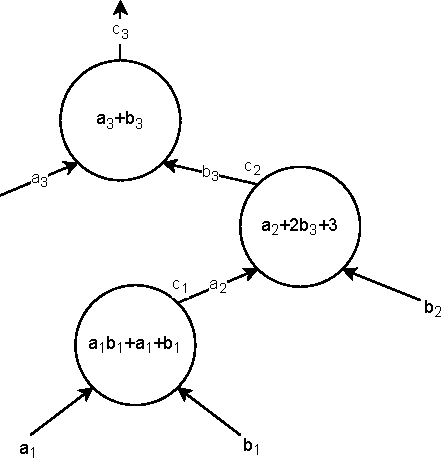
\includegraphics[width=0.4\textwidth]{../figures/plonk-circuit.drawio}
\caption{Example of a \plonk-like circuit.}
\label{figure:plonk-circuit-example}
\end{figure}

Observe all the values below depend only on the shape of the circuit itself, so if the circuit does not change, this polynomial should not be recomputed. Check that the \SA, \SB and \SC polynomials are constructed so that we can verify the copy-constraints $c_2 = b_3$ and $c_1 = a_2$ present in the circuit. Observe that equally painted cells have their values swapped, as explained before in the construction of the connection $S$ polynomials.  

\begin{figure}[H]
\centering
\begin{tabular}{|c|c|c|c|c|c|c|c|}
\hline
\QL	&\QR	&\QM	&\QO	&\QC	&\SA					&\SB						&\SC 							\\ \hline
1			&1				&1				&-1				&0				&1								&$k_1$								&\cellcolor{pink} $g$				\\
1			&2				&0				&-1				&3				&\cellcolor{pink}$k_2$			&$k_1 \cdot g$					&\cellcolor{cyan} $k_1 \cdot g^2$	\\
1			&1				&0				&-1				&0				&$g^2$						&\cellcolor{cyan}$k_2 \cdot g$ &$k_2 \cdot g^2$					\\
\hline
\end{tabular}
\label{table:plonk-circuit-example}
\end{figure}

Therefore, we can derive a PIL program that validates the previous circuit as shown below:
\begin{pil}
include "config.pil";

namespace Plonk(%N);
    pol constant QL, QR, QM, QO, QC;
    pol constant SA, SB, SC;
    pol constant L1;
    
    pol commit a, b, c;
    
    public pi = a(0);
    
    // Public values check 
    L1 * (a - :pi) = 0;
    
    // Plonk equation 
    pol ab = a*b;
    QL*a + QR*b + QM*ab + QO*c + QC = 0;

    // Copy-constraints check 
    {a, b, c} connect {SA, SB, SC};
\end{pil}




%%%%%%%%%%%%%%%%%%%%%%%%%%%%%%%%%%%%%%%%%%%%%%%%%%%%%%%%%%%%%%%%
\subsection{Filling Polynomials}

Until now we have only shown how to specify some kinds of constraints that several polynomials of a certain program described in PIL should satisfy to become \textit{correct}. All these constraints, together with the constant polynomials inherent to the computation itself, specify the transition function underlying the program definition. In other words, changing either any of the constraints or the description of the constant polynomials produces a change in the program we are working on. 

%TODO Check this paragraph
In this section, we are going to use Javascript and \pilcom to generate a specific execution trace for a given PIL. To do so, we are going to compute a valid execution trace for the example of Section \ref{sec:connecting-sm}. As a remark, we will also use the library \texttt{pil-stark} whose utility is to provide a framework to setup, generate and verify proofs, to use a \texttt{FGL} class which mimics a finite field and it is required by some functions that provide the \pilcom package. 

First of all, under the scope of an asynchronous function called \texttt{execute}, we parse the provided PIL (which is, in our case, \texttt{main.pil}) into a Javascript object using the \texttt{compile} function of \pilcom. In code we obtain:
\begin{js}
const { FGL } = require("pil-stark");
const { compile } = require("pilcom");
const path = require("path");

async function execute() {
    const pil = await compile(FGL, path.join(__dirname, "main.pil"));
}
\end{js}

The \pilcom package also provides two functions that use the \texttt{pil} object to create two crucial objects from it for the construction of the execution trace: the constant polynomials object and the committed polynomials object (using \texttt{newConstPolsArray} and \texttt{newCommitPolsArray} functions, respectively).
\begin{js}
const { newConstantPolsArray, newCommitPolsArray, compile } = require("pilcom");

async function execute() {

    // ... Previous Code
    
    const constPols =  newConstantPolsArray(pil);
    const cmPols = newCommitPolsArray(pil);
}
\end{js}

Both such objects contain useful information about the PIL itself, such as the provided length of the program $N$, the total number of constant polynomials and the total number of committed polynomials. However, accessing these objects will allow us to fill the entire execution trace for that PIL. We can access a specific position of the execution trace using the syntax:
\begin{js}
pols.Namespace.Polynomial[i] 
\end{js}
being \texttt{pols} one of the previously introduced \texttt{constPols} and \texttt{cmPols} objects, \texttt{Namespace} being a specific namespace among the ones defined by the PIL files, \texttt{Polynomial} one of the polynomials defined under the scope of the previous namespace and $i$ an integer in the set $[0,N-1]$ representing the row of the current polynomial. Using this we can now start to fill our polynomials. 

In our example, we will use, as inputs for the trace, which are the ones introduced in the \texttt{Main.a} polynomial, an ascending chain of integers from $0$ to $15$ cyclically (because recall that we are only allowed to use $4$ bits integers). We propose here two functions that fill the constant and committed polynomials accordingly. 
\begin{figure}[H]
\begin{js}
async function buildConstantPolynomials(constPols, polDeg) {
    
    for (let i=0; i < polDeg; i++) {
        constPols.Global.BITS4[i] = BigInt(i & 0b1111);
        constPols.Global.L1[i] = i === 0 ? 1n : 0n;
        constPols.Negation.RESET[i] = (i % 4) == 3 ? 1n : 0n;
        constPols.Negation.FACTOR[i] = BigInt(1 << (i % 4));
        constPols.Negation.ISLAST[i] = i === polDeg-1 ? 1n : 0n;
    }
}
\end{js}
\caption{Generation of the constant polynomials.}
\end{figure}

\begin{figure}[H]
\begin{js}
async function buildcommittedPolynomials(cmPols, polDeg) {
        
    cmPols.Negation.a[-1] = 0n;
    cmPols.Negation.neg_a[-1] = 1n;
    
    for (let i=0; i < polDeg; i++) {
        
        let fourBitsInt = i % 16;
        
        cmPols.Main.a[i] = BigInt(fourBitsInt);
        cmPols.Main.neg_a[i] = BigInt(fourBitsInt ^ 0b1111);
        cmPols.Main.op[i] = FGL.mul(cmPols.Main.a[i], cmPols.Main.neg_a[i]);
        
        cmPols.Multiplier.freeIn1[i] = cmPols.Main.a[i];
        cmPols.Multiplier.freeIn2[i] = cmPols.Main.neg_a[i];
        cmPols.Multiplier.out[i] = cmPols.Main.op[i];
        
        let associatedInt = Math.floor(i/4);
        let bit = (associatedInt >> (i%4) & 1) % 16;
        cmPols.Negation.bits[i] = BigInt(bit);
        cmPols.Negation.nbits[i] = BigInt(bit ^ 1);
        
        
        let factor = BigInt(1 << (i % 4));
        let reset = (i % 4) == 0 ? 1n : 0n;
        cmPols.Negation.a[i] = factor*cmPols.Negation.bits[i] 
        + (1n-reset)*cmPols.Negation.a[i-1];
        cmPols.Negation.neg_a[i] = factor*cmPols.Negation.nbits[i] 
        + (1n-reset)*cmPols.Negation.neg_a[i-1];
    }
}
\end{js}
\caption{Generation of the committed polynomials.}
\end{figure}

Now that we have all the constant and committed polynomials filled in, we can check using a function called \texttt{verifyPil} that they indeed satisfy the constraints defined in the PIL file. We provide below the piece of code that construct the polynomials and check the constraints. If the verification procedure fails, we should not proceed to the proof generation because it will lead to false proof. 
\begin{js}
const { newConstantPolsArray, newCommitPolsArray, compile, verifyPil } = require("pilcom");
    
async function execute() {
    
    // ... Previous Code	
    
    const N = constPols.Global.BITS4.length;
        
    await buildConstantPolynomials(constPols, N);
    await buildcommittedPolynomials(cmPols, N);
    
    const res =  await verifyPil(FGL, pil, cmPols , constPols);
    if (res.length != 0) {
        console.log("The execution trace do not satisfy PIL restrictions. Aborting...");
        for (let i=0; i<res.length; i++) {
            console.log(res[i]);
            return;
        }
    }
}
\end{js}







%TODO: Is this section necessary?
%%%%%%%%%%%%%%%%%%%%%%%%%%%%%%%%%%%%%%%%%%%%%%%%%%%%%%%%%%%%%%%%%
\subsection{Generating a Proof Using \texttt{pil-stark}}

Once the constant and the committed polynomials are filled, we can step to the proof generation stage. We can use the \texttt{pil-stark} Javascript package specially designed to work together with \pilcom in order to generate STARK proofs about PIL statements. We will use three functions \texttt{starkSetup}, \texttt{starkGen} and \texttt{starkVerify} from the package. The first one is aiming for setting up the STARK, which is independent from the values of committed polynomials. This includes the computation of the tree of the evaluations of the constant polynomials. For executing the setup generation we ought to have an object called \texttt{starkStruct} which is specifying several FRI-related parameters such as the size of the trace domain (which must coincide with $N$, defined in PIL), the size of the extended domain (which together with the previous parameter specifies the correspondent \textit{blowup factor}), the number of queries to be executed and the reduction factors for each of the FRI steps. We execute the setup using the code below:

\begin{js}
const { FGL, starkSetup } = require("pil-stark");
    
async function execute() {
    
    // ... Previous Code	
    
    const starkStruct = {
        "nBits": 10,
        "nBitsExt": 11,
        "nQueries": 128,
        "verificationHashType": "GL",
        "steps": [
        {"nBits": 11},
        {"nBits": 5},
        {"nBits": 3},
        {"nBits": 1}
        ]
    };
        
    const setup = await starkSetup(constPols, pil, starkStruct);
}
\end{js}

Now that we have set up the STARK, we can generate the proof using the \texttt{starkGen} function. We can do this task using the code below. Observe that the \texttt{setup} object contains inside a \texttt{starkInfo} field which contains, aside from all the \texttt{starkStruct} parameters, lots of useful information about the shape of the PIL itself. 

\begin{js}
const { FGL, starkSetup, starkGen } = require("pil-stark");

async function execute() {
    
    // ... Previous Code	
    
    const resProof = await starkGen(cmPols, constPols, setup.constTree, setup.starkInfo);
}
\end{js}

Now that a proof has been generated we can be involved in the verification procedure invoking the \texttt{starkVerify} function. This function needs, as arguments, some information provided by the outputs of both the \texttt{starkSetup} and \texttt{starkGen} functions. If the output of the \texttt{starkVerify} function is \texttt{true}, the proof is valid. Otherwise, the verifier should invalidate the proof sent by the prover. 

\begin{js}
const { FGL, starkSetup, starkGen, starkVerify } = require("pil-stark");
    
async function execute() {
        
    // ... Previous Code
    
    const resVerify = await starkVerify(
        resP.proof, resP.publics, setup.constRoot, setup.starkInfo
    );
    
    if (resVerify === true) {
    console.log("The proof is VALID!");
    } else {
    console.log("INVALID proof!");
    }
}
\end{js}












%%%%%%%%%%%%%%%%%%%%%%%%%%%%%%%%%%%%%%%%%%%%%%%%%%%%%%%%%%%%%%%
\section{TODO: Use Cases}





%%%%%%%%%%%%%%%%%%%%%%%%%%%%%%%%%%%%%%%%%%%%%%%%%%%%%%%%%%%%%%%
\section{TODO: Conclusions} 
